\newpage
\chapter{Verification and Validation}
\label{ch-VandV}


\iffalse

(Units        = lowest level functions testing. Function testing implemented as a framework --> super brief)
--> (sub-)module = functions calling functions. System test --> verification with literature or sensitivity <--


\fi


Having developed tools as complex as presented (see flowchart \autoref{sec:toolintegration}), it is important to verify and validate the components as well as the integration to be able to fully rely on it when applying it in concept decisions or further design work. Different strategies are therefore devised: Every subpart of the tool can be verified using module tests with simplified inputs and known outputs (\autoref{sec:veriTools}). In \autoref{sec:sensiForTesting} it is explained how the sensitivity analysis tool (\autoref{sec:sensitivityplot}) was applied to check the integration of the subtools. Furthermore, \autoref{sec:errorSensitivity} contains analysis of estimation errors due to assumptions using the same sensitivity framework. Finally, an intermediate design validation is shown in section \ref{sec:statsVal} linking the designs to known statistics.


\section{Verification of existing tools} \label{sec:veriTools}

Many of the tool components shown in \autoref{CriteriaTools} are verified using tests with (possibly simplified) inputs and outputs known from hand calculations, other academic research or otherwise known. These are presented here for the BEMT (\autoref{sec:BEMTVerification}), Noise (\autoref{sec:NoiseVerification}), Downwash (\autoref{sec:DownwashVerification}), Route selection \& passenger throughput (\autoref{sec:RouteSelVerification}), system size estimation (\autoref{sec:SysSizeVerification}) and ATC efforts (\autoref{sec:ATCVerification}).



\subsection{BEMT}  \label{sec:BEMTVerification}

To verify the tool, the Harrington 1 coaxial rotor parameters were input into the tool, and the results for radial distribution of inflow, power/torque and thrust coefficients were compared at torque balance and a uniform pitch distribution (no twist) of 8 degrees. The comparison is shown in  \autoref{fig:verification_thrust} for the thrust coefficients. 

There is almost an identical correspondence for the inflow distribution and thrust coefficient plots. However, the power coefficients in the implemented BEMT seem to be overestimated (even though they have the correct order of magnitude). This means that for a fixed value of thrust required from a rotor, the torque required will be overestimated, which will increase the noise signature.

After quantifying the effect of this inaccuracy on the outputs of the tool which are design criteria (such as noise), it will be decided how much effort should go into improving the accuracy of the current BEMT.

\begin{comment}

\begin{figure}
\captionsetup[subfigure]{justification=centering}
\begin{subfigure}[t]{0.5\textwidth}
    \centering
    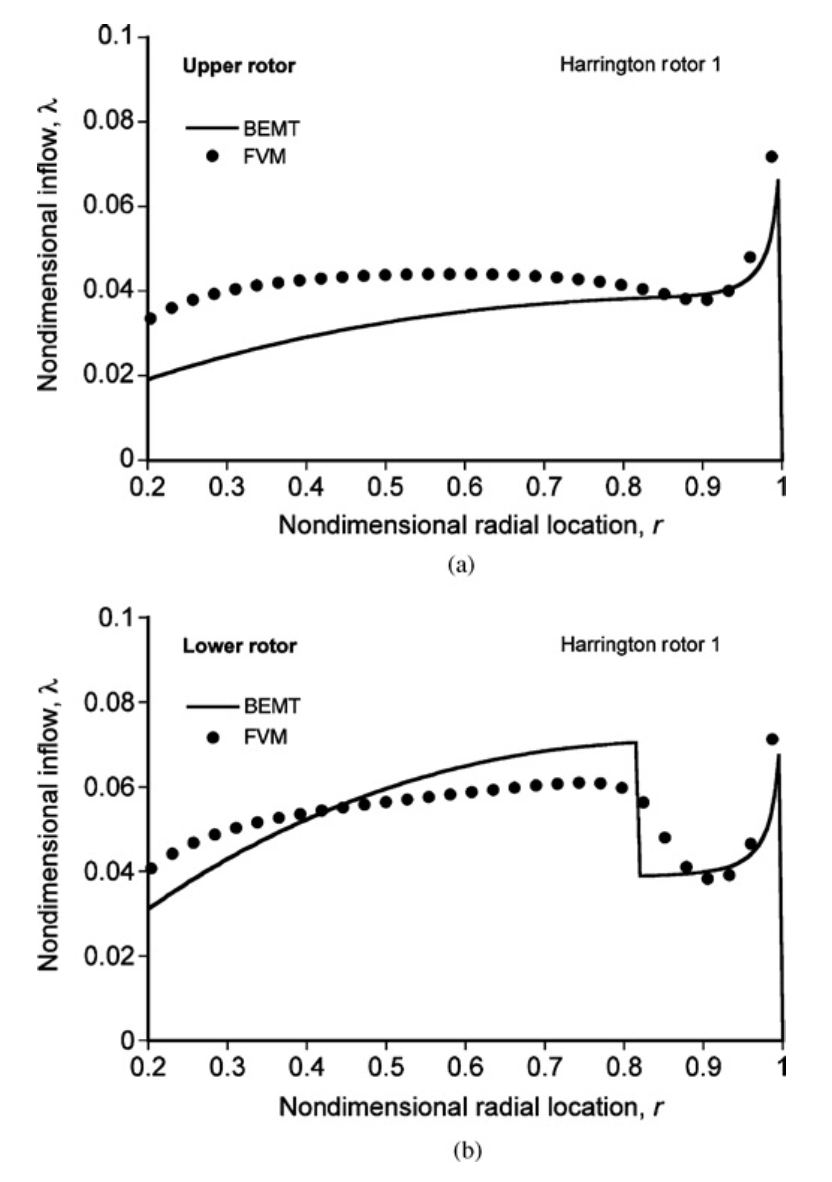
\includegraphics[width=\textwidth]{Figures/Leishman_inflow.png}
    \caption{Spanwise inflow distribution prediction by the BEMT in \cite{BEMT} and the Maryland Free Vortex Model in hover (torque balance)}
    %\label{fig:blade2d}
\end{subfigure}
\begin{subfigure}[t]{0.5\textwidth}
    \centering
    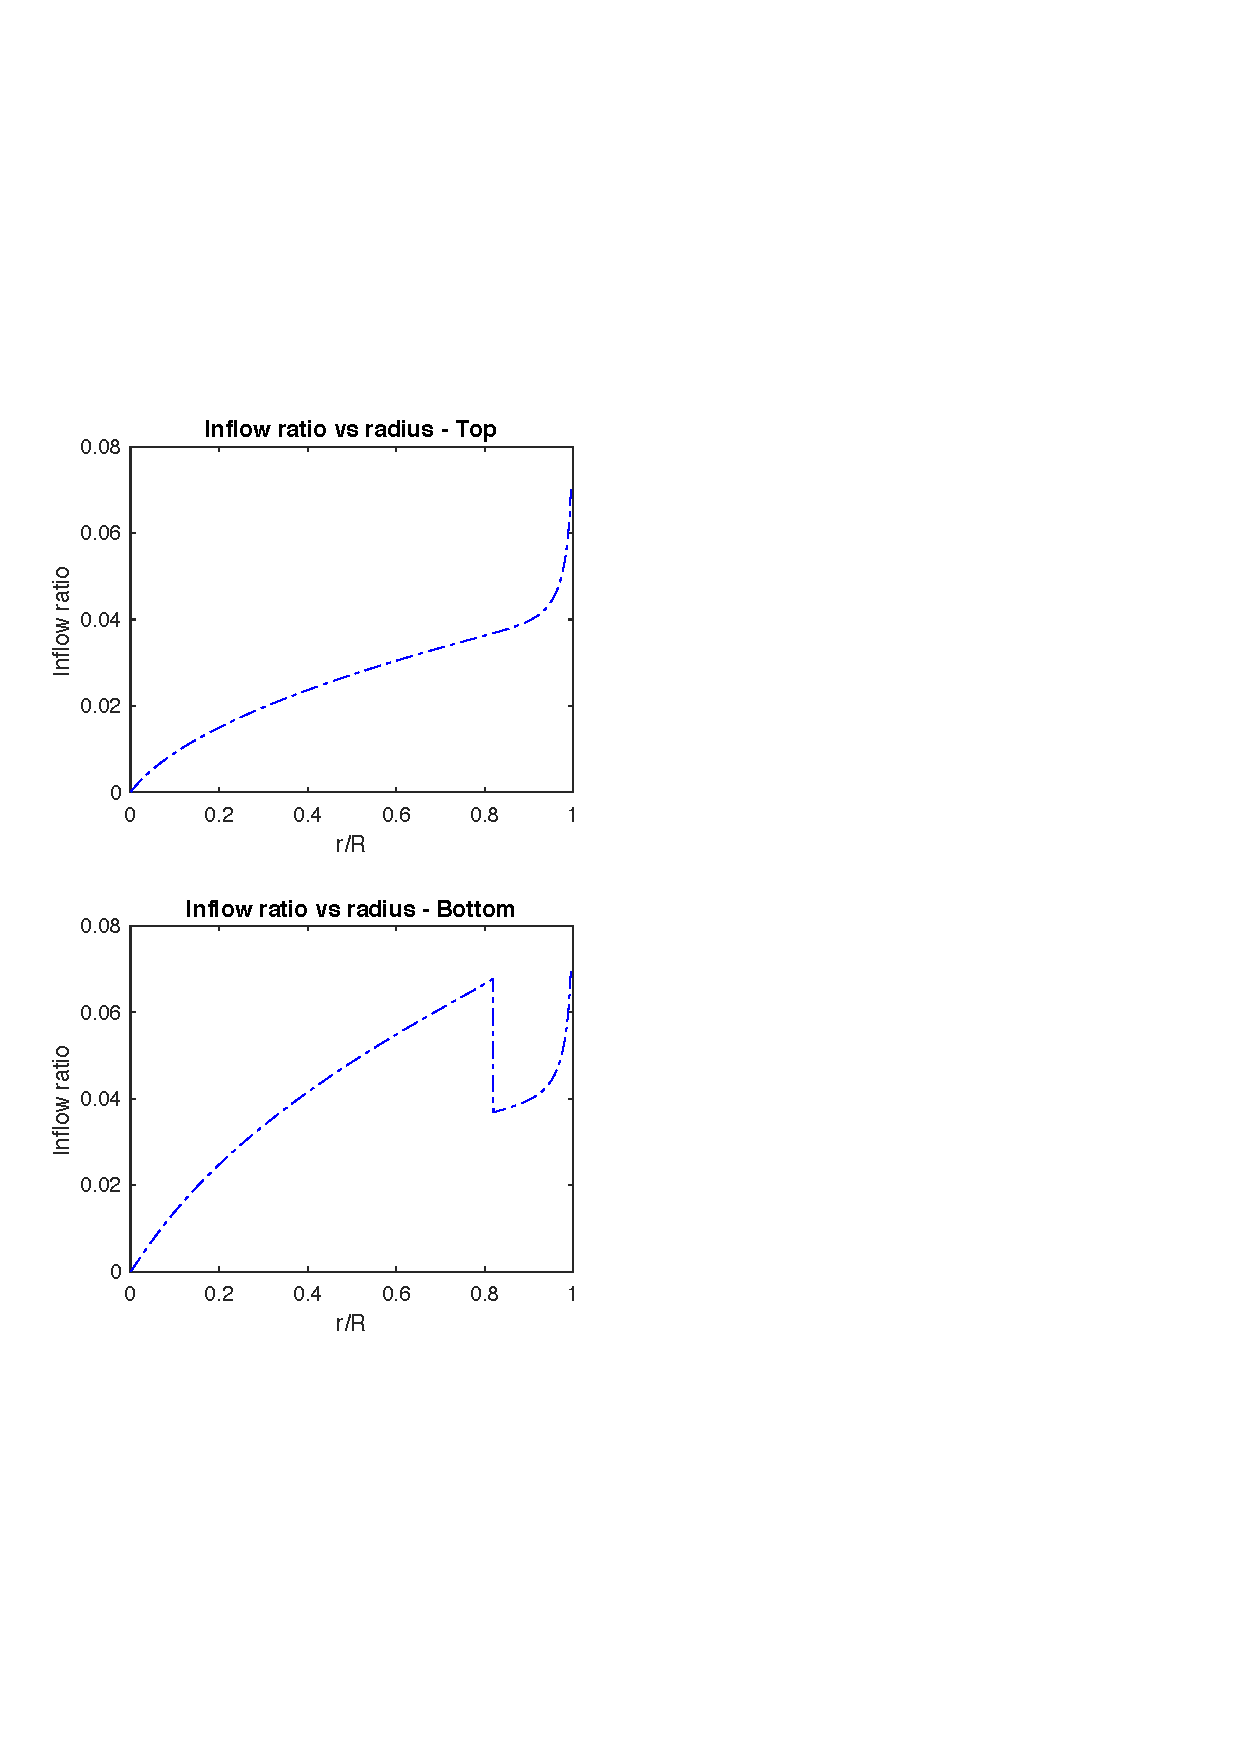
\includegraphics[width=\textwidth]{Figures/verification_inflow.pdf}
    \caption{Spanwise power coefficient prediction by implemented BEMT tool in hover (torque balance)}
    %\label{fig:disks}
\end{subfigure}
    \captionsetup{justification=centering}
    \caption{Verification plots for upper and lower rotor inflow distribution prediction of the Harrington 1 rotor.}
    \label{fig:verification_inflow}
\end{figure}

\end{comment}

\begin{figure}
\captionsetup[subfigure]{justification=centering}
\begin{subfigure}[t]{0.5\textwidth}
    \centering
    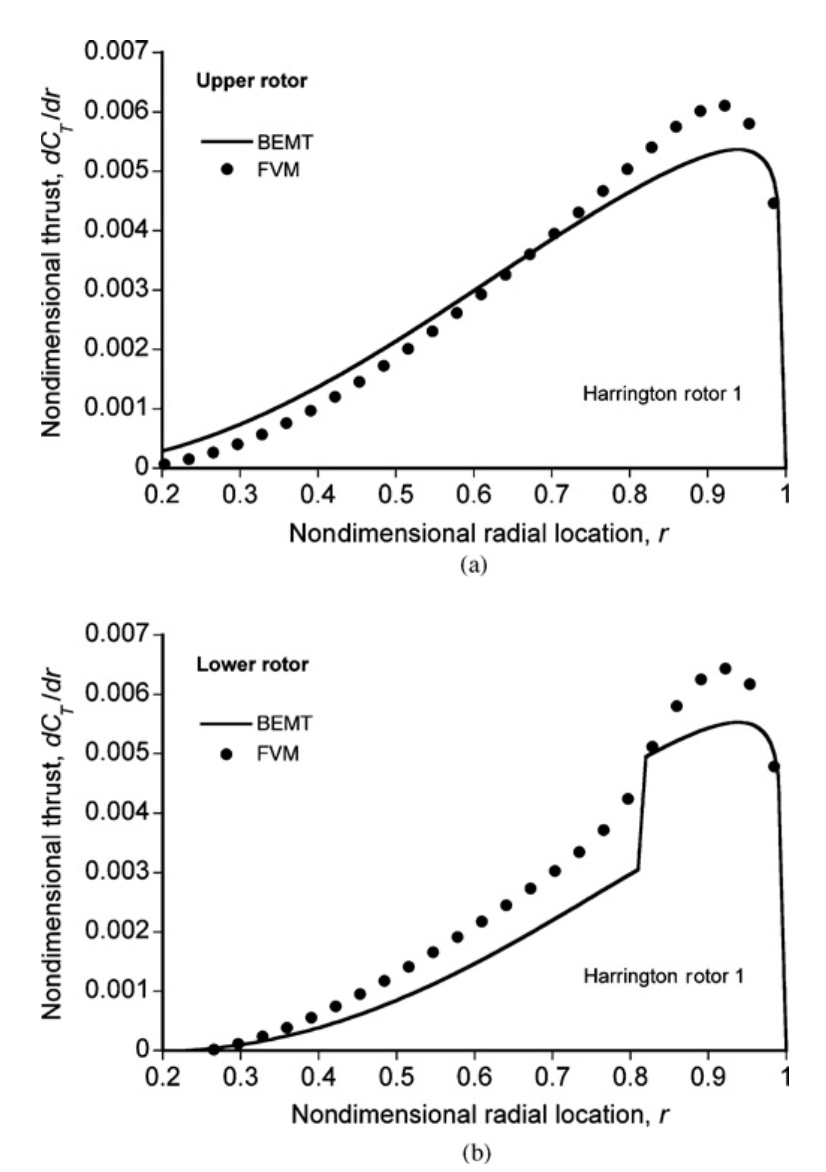
\includegraphics[width=\textwidth]{Figures/Leishman_CT.png}
    \caption{Spanwise thrust coefficient prediction by the BEMT in \cite{BEMT} and the Maryland Free Vortex Model in hover (torque balance)}
    %\label{}
\end{subfigure}
\begin{subfigure}[t]{0.5\textwidth}
    \centering
    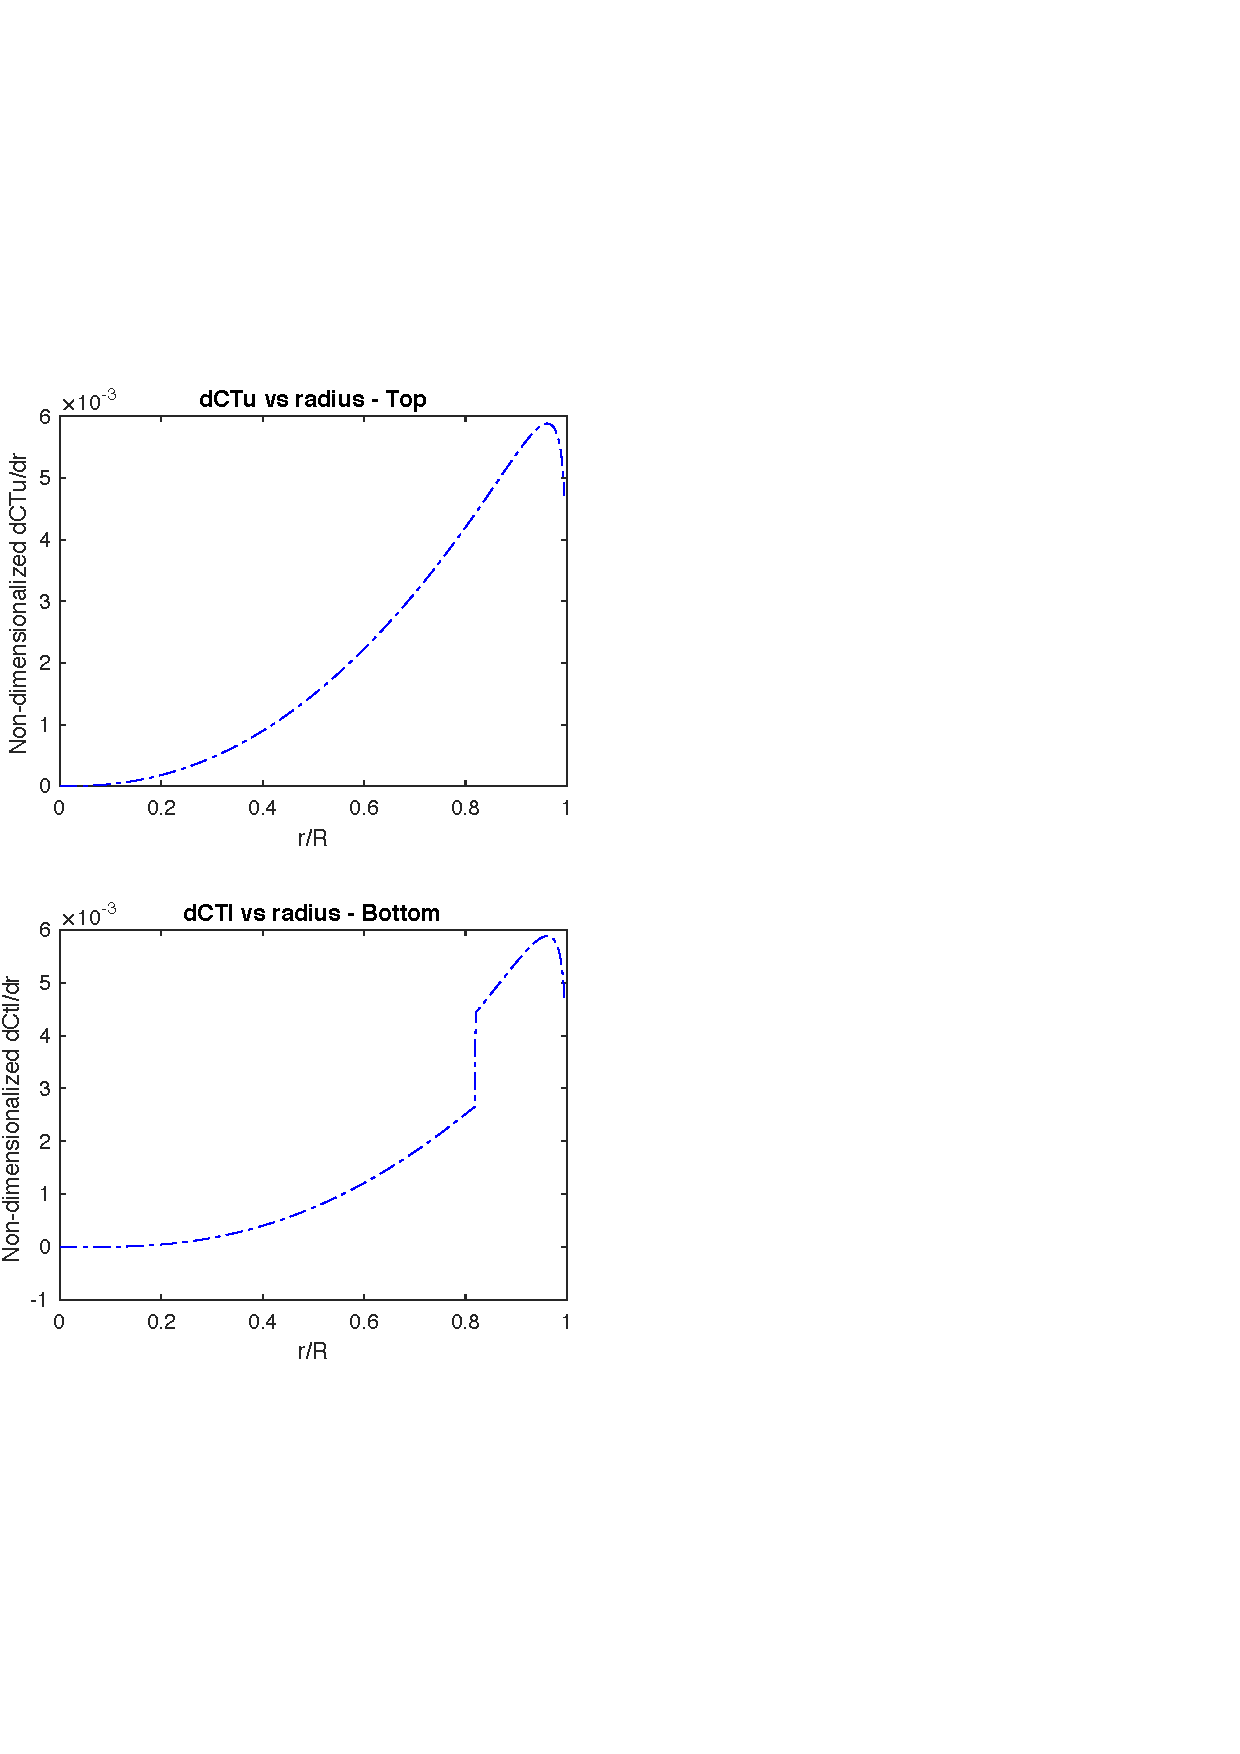
\includegraphics[width=\textwidth]{Figures/CT_plot.pdf}
    \caption{Spanwise power coefficient prediction by implemented BEMT tool in hover (torque balance)}
    %\label{fig:disks}
\end{subfigure}
    \captionsetup{justification=centering}
    \caption{Verification plots for upper and lower rotor thrust coefficient prediction of the Harrington 1 rotor.}
    \label{fig:verification_thrust}
\end{figure}

\begin{comment}


\begin{figure}
\captionsetup[subfigure]{justification=centering}
\begin{subfigure}[t]{0.5\textwidth}
    \centering
    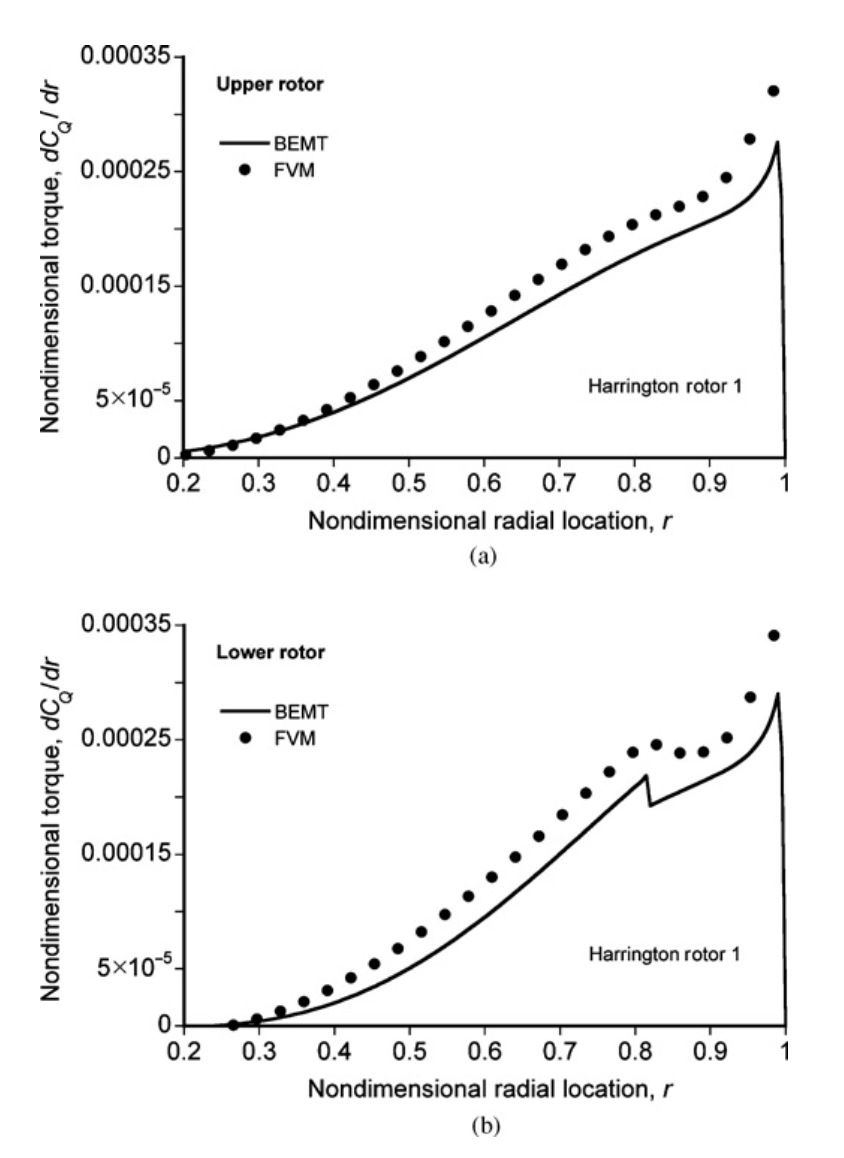
\includegraphics[width=\textwidth]{Figures/Leishman_CP.png}
    \caption{Spanwise power coefficient prediction by the BEMT in \cite{BEMT} and the Maryland Free Vortex Model in hover (torque balance)}
    %\label{fig:blade2d}
\end{subfigure}
\begin{subfigure}[t]{0.5\textwidth}
    \centering
    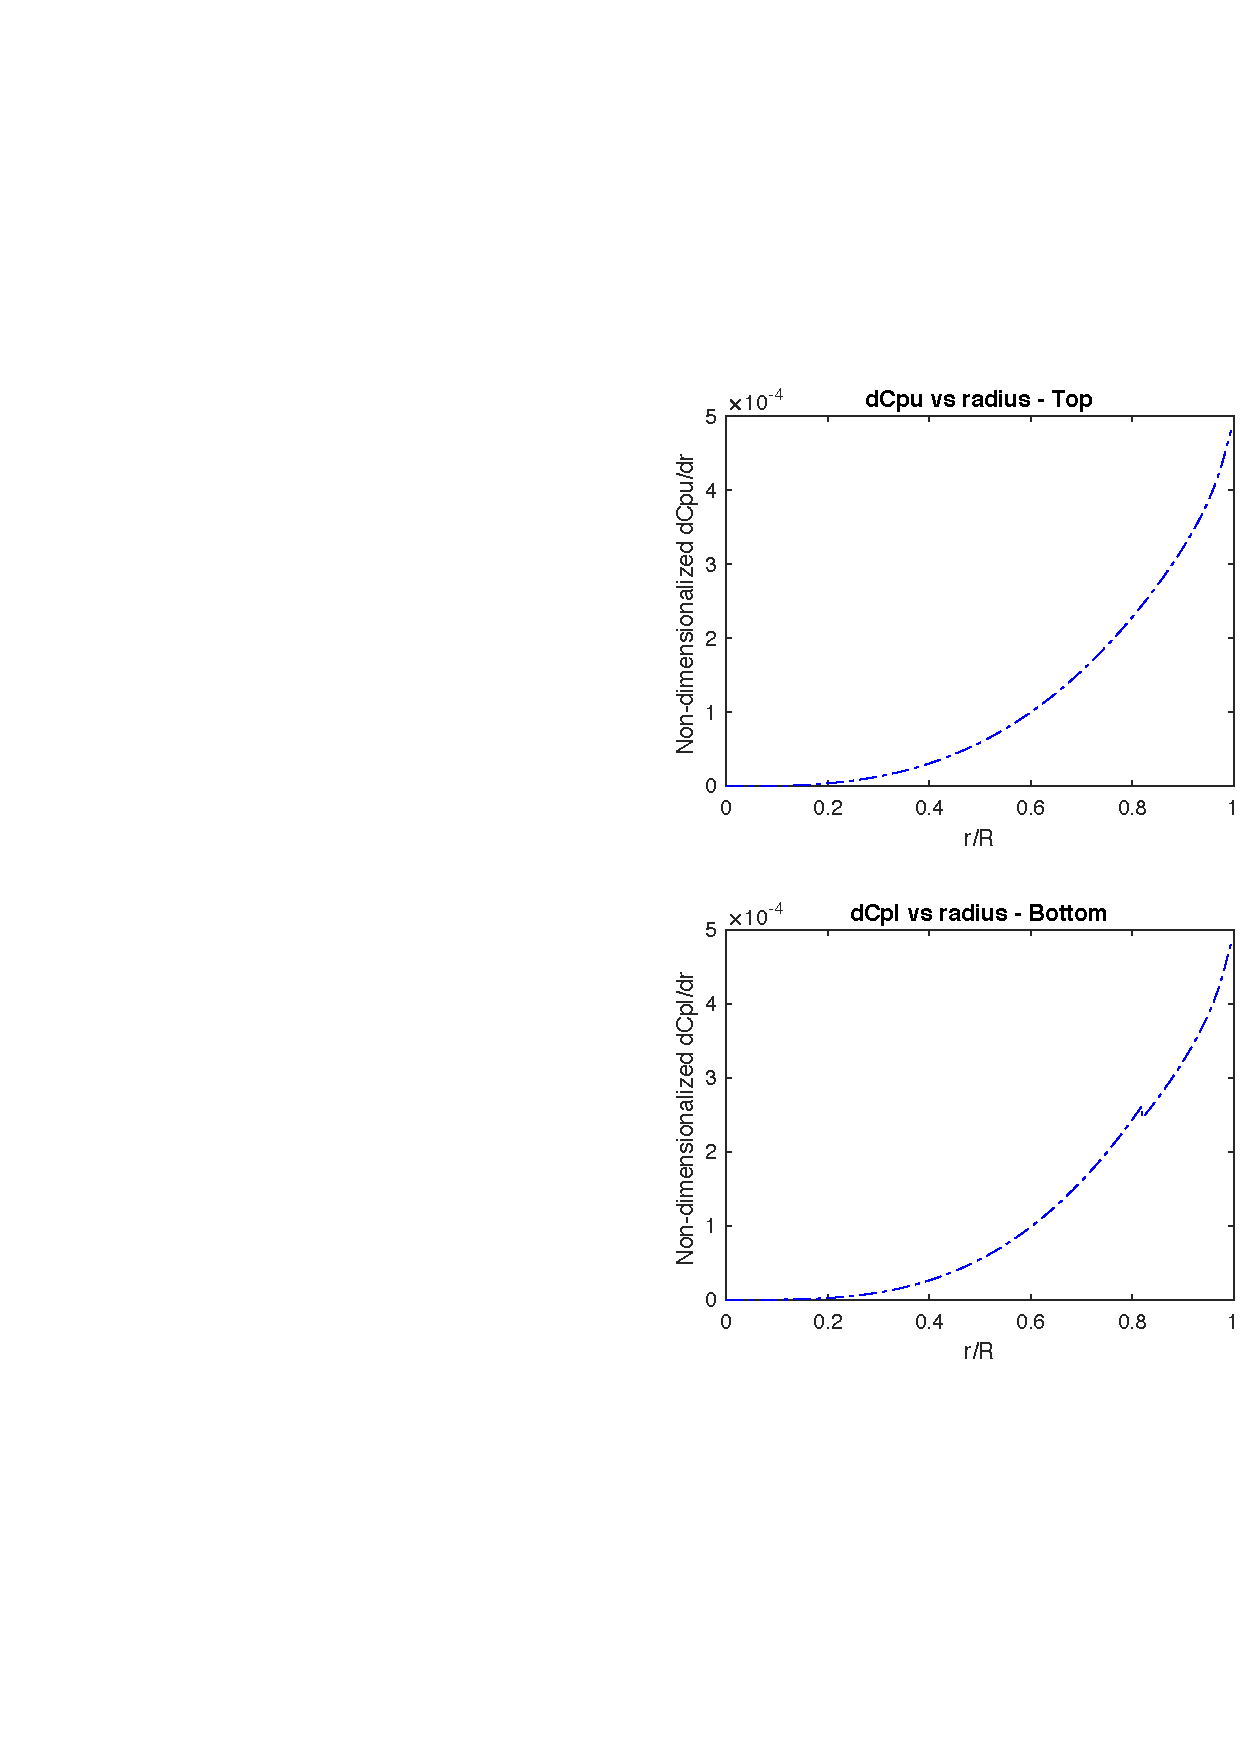
\includegraphics[width=\textwidth]{Figures/CP_plot.pdf}
    \caption{Spanwise power coefficient prediction by implemented BEMT tool in hover (torque balance)}
    %\label{fig:disks}
\end{subfigure}
    \captionsetup{justification=centering}
    \caption{Verification plots for upper and lower rotor power coefficient prediction of the Harrington 1 rotor.}
    \label{fig:verification_torque}
\end{figure}

\end{comment}

\subsection{Noise} \label{sec:NoiseVerification}

A thorough verification as done for the BEMT tool could not be performed due to time constraints. However, the article that the tool is based on does provide the parameters of the vehicles in the study and their noise signature, which will be used in the future to verify the accuracy of the tool. That being said, the outputs of the tool have realistic magnitudes and seem to behave as expected. For instance, the sensitivities of MTOW and noise always show that the noise increases when the MTOW increases, which is intuitively logical and can be extracted from the equations presented above. For vehicles with rotors that have low fundamental frequencies the noise footprint in dBA is lower than in dB, which also makes sense if one looks at the A-weighting curve which peaks at around 3 kHz. Many more of these sanity checks have been performed during tool integration and show up in the sensitivity studies. However, due to report space constraints, the plots for these sensitivities are not shown.

\subsection{Downwash} \label{sec:DownwashVerification}

The downwash tool is fairly concise so the verification of this tool is trivial. Several unit tests can be performed. The first one is to double check whether the computed thrust makes sense, by looking at the computed values and the signs that are obtained. The next is to look if the found air velocities are correct. Here it is, just as in the thrust case, important to verify the sign. A positive flow velocity is defined as the case where the air moves through the rotor from up to down. The same holds for the mass flow. After these test are performed, the workings of the tool as a whole are verified by entering some extreme values, like zero and very large numbers, to check if the software does not report any errors and gives the expected values (e.g. zero thrust should not produce an induced flow field and thus zero downwash velocity).   

\subsection{Route Selection and Passenger Throughput Requirement} \label{sec:RouteSelVerification}

Since only $40\ 000$ of Google Maps API Directions queries were available free of charge from Google and $14\ 000$ are needed, care must be taken to verify the queries before issuing them to mitigate the risk of using up the queries accidentally without obtaining useful results. This was done by requesting the same information for a few randomly chosen trips manually on \url{www.google.com/maps} and via the API from MATLAB. After this succeeded and the information was confirmed to be identical, the integration was checked by using the final input and output files, but limiting the trips to 5 at random. Following this, a dry run was performed by formulating all queries and writing the output files as before, but without actually invoking the API. 

After enough confidence was established, the program ran in around 2 hours. However, when evaluating the average time loss due to traffic, the percentage (33\% of average trip time added) did not match the TomTom traffic index \footnote{\url{https://www.tomtom.com/en_gb/trafficindex/city/los-angeles} [accessed 21.05.19]} which reports 62\% for the morning peak in 2016 (with an upwards trend in the recent years), at the same time of day as predicted by this algorithm (8am to 9am). To investigate this, the traffic model that Google provides was configured from "best-estimate" to "pessimistic". This overestimated the average trip time added as 80\% which is closer to the TomTom data.

To verify the flux calculations, a shortened trip definitions file was created and the fluxes manually computed for the low amount of trips. This was compared and confirmed to match with the scripted calculations and also associativity with the GEOIDS (specifying the location within LA country) was confirmed to be kept. Although not shown here for brevity, these unit testing files are available from us on request.

\subsection{System Size Estimation and Daily Footprint} \label{sec:SysSizeVerification}

Correct operation of the tool integration needs to be confirmed, especially with regards to keeping the associativity of the PUMAs and treating the route inverses correctly. This was achieved by inputting a trip database of only two trips with 100 passengers going one way on a route and 60 passenger going to opposite way on the same route, at each time of the day. The smaller database allowed to do hand calculations with which to compare the tool outputs. $\zeta$ was set to $1$ initially and then varied.

After correcting a forgotten ceiling function in calculation of the number of gates, the results matched one-to-one when comparing all six quantities above (which caused a few percent of relative error), which increases confidence in the implementation.

\subsection{ATC Efforts} \label{sec:ATCVerification}

The ATC efforts tool was the last tool to be created and therefore little verification effort has been invested in it. However, built-in functions have been used where possible and edge cases have been identified for calculating the number of intersections and the number of vehicle conflicts. An edge case that has to be solved when calculating the number of intersections is when multiple routes converge to a single point (which is currently being counted as an intersection but it is not). An edge case for the number of conflicts is when intersecting trips have a different number of vehicles travelling through them, where instead of summing the number of vehicles along the routes, the minimum number of vehicles on both routes should specify the number of potential conflicts.
















\section{Sensitivity Analysis for System Testing} \label{sec:sensiForTesting}

In the section above, the verification method of each module of the tool has been presented. However, the correct integration of the modules into the umbrella tool also had to be checked. This was done in two ways: first, every team member was given access to the tool and was allowed to input vehicle concepts into it. Having 10 students testing the tool allowed us to quickly find limitations and edge cases where it would not work (either it would crash or not converge on certain iterations). Another effective method of performing system tests of the tool was to perform sensitivity plots (see \autoref{sec:sensitivityplot}) of the outputs with the inputs. This very quickly allowed us to check if the input-output relation between parameters (e.g. maximum dimension of vehicle and pad cost) was what one would expect (in this case a positive correlation). The example given above is a very obvious one, but in some cases (like ticket price vs battery energy density) the tool showed counter-intuitive relations which after some thought could be explained.

This section provides the reader with some specific examples of the above concepts that should increase the faith in the toolchain developed.


\subsection{Pad Costs}
It was determined that the pad cost could be a major driver of ticket price. The initial assumption was that the ground area needed for the vertiports in downtown LA would have similar cost to office space. If this is the case, over 80\% of the ticket price goes just to these rental fees. This can be seen in \autoref{fig:sens01}. The black x's in the plot show the operating cost without any pad costs. Ideally, better cost arrangements or business models can be developed to subsidise or eliminate the pad cost.


\subsection{Minimum Trip Range}
By limiting the trip range to a certain minimum, there are two effects that cause the ticket price to drop as shown in \autoref{fig:sens02}. First, the trip efficiency increases if no short trips are allowed (shown in \autoref{fig:sens03}), which reduces energy cost. In addition, due to the calculation method of the tool, a limited trip range means a larger market share is required. Naturally, a larger market share allows for a lower ticket price in the long run. 

\autoref{fig:sens1} shows that, when the minimum range is increased, the total system area increases due to the increased market share. This would increase the pad costs (driving ticket price), but the increased market share still allows for a reduction of the final ticket price. 

When increasing the last-mile penalty, the market share increases, as shown in \autoref{fig:sens2}. Intuitively, it should reduce the market share, as a bigger last-mile penalty would normally decrease demand for flying (as it would take longer to get to and from the vertiport). However, the tool adjusts the market share to meet a standard time savings.

Going forward, the demand must be considered to determine how much market share will be possible in reality. This is an important risk to consider, as it drives the final success of the system. The current tool assumes that demand is essentially infinite, but in reality is likely to be tied directly to trip range and last-mile penalty.


\begin{figure}[h]
\begin{subfigure}[t]{0.33\textwidth}
    \centering
    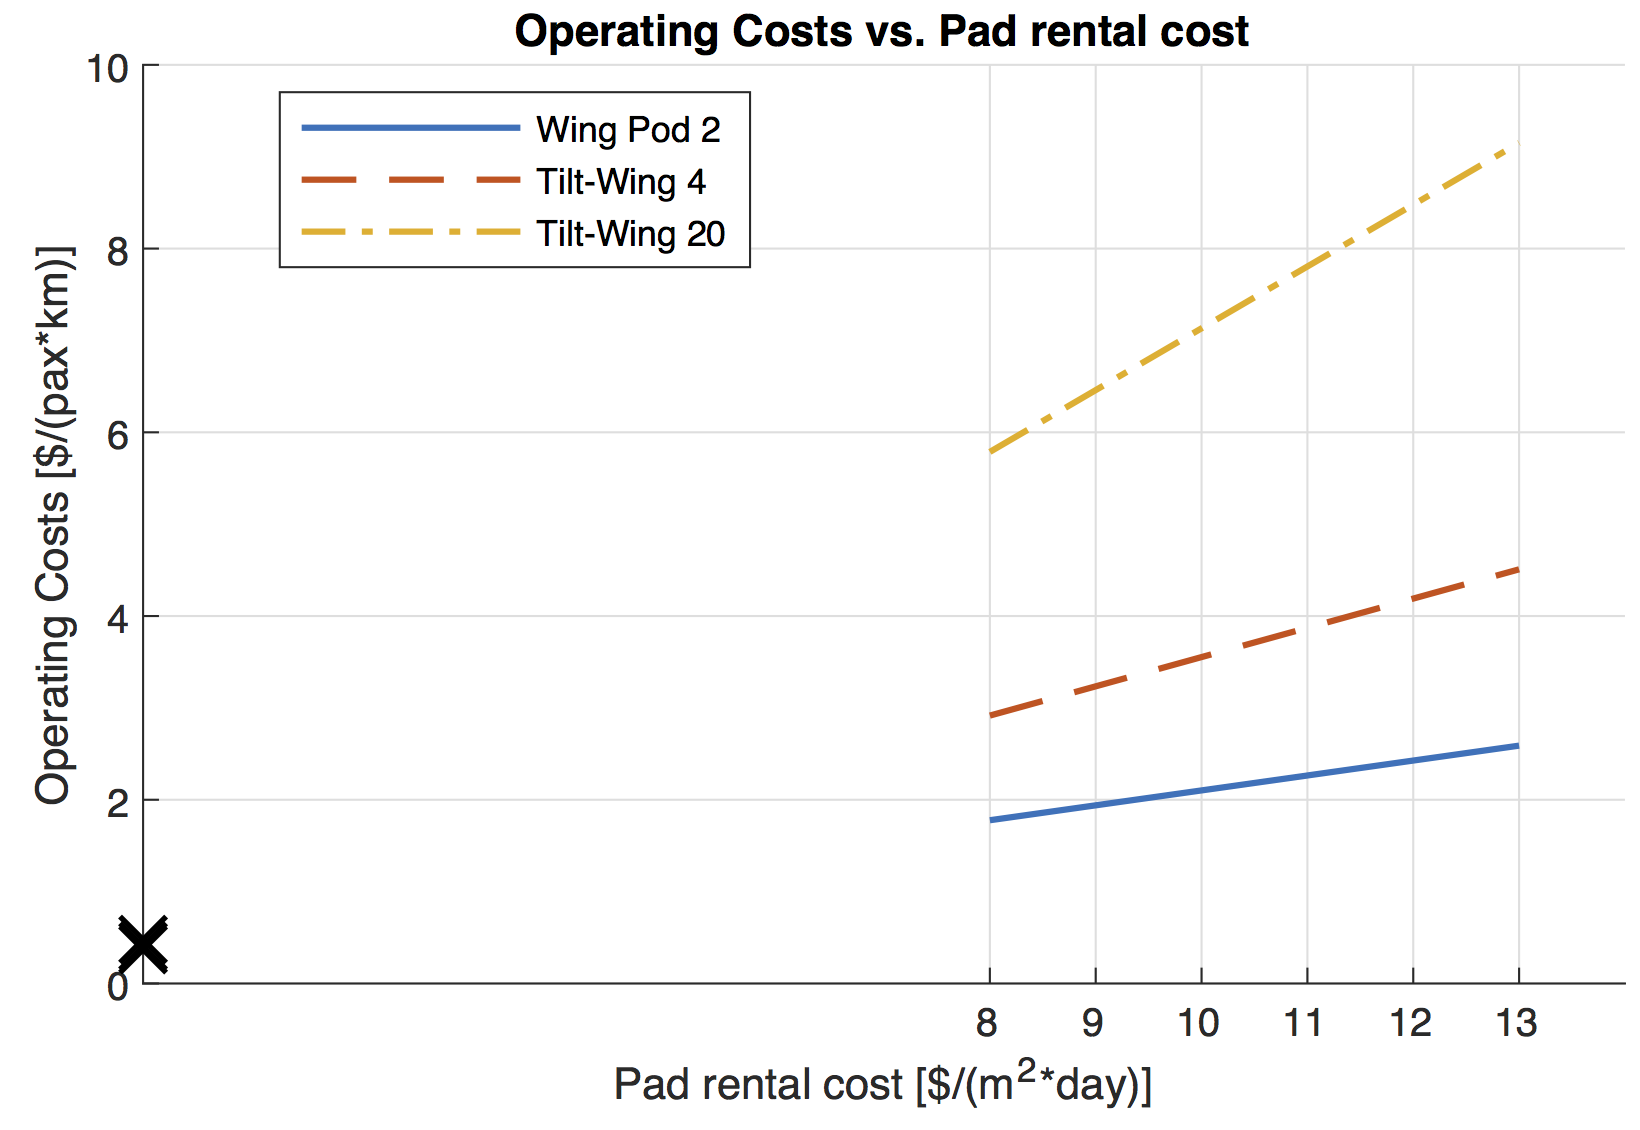
\includegraphics[width=\textwidth]{Figures/cost_oper.png}
    \captionsetup{justification=centering}
    \caption{Total operating cost vs. Pad rental costs}
    \label{fig:sens01}
\end{subfigure}
\begin{subfigure}[t]{0.33\textwidth}
    \centering
    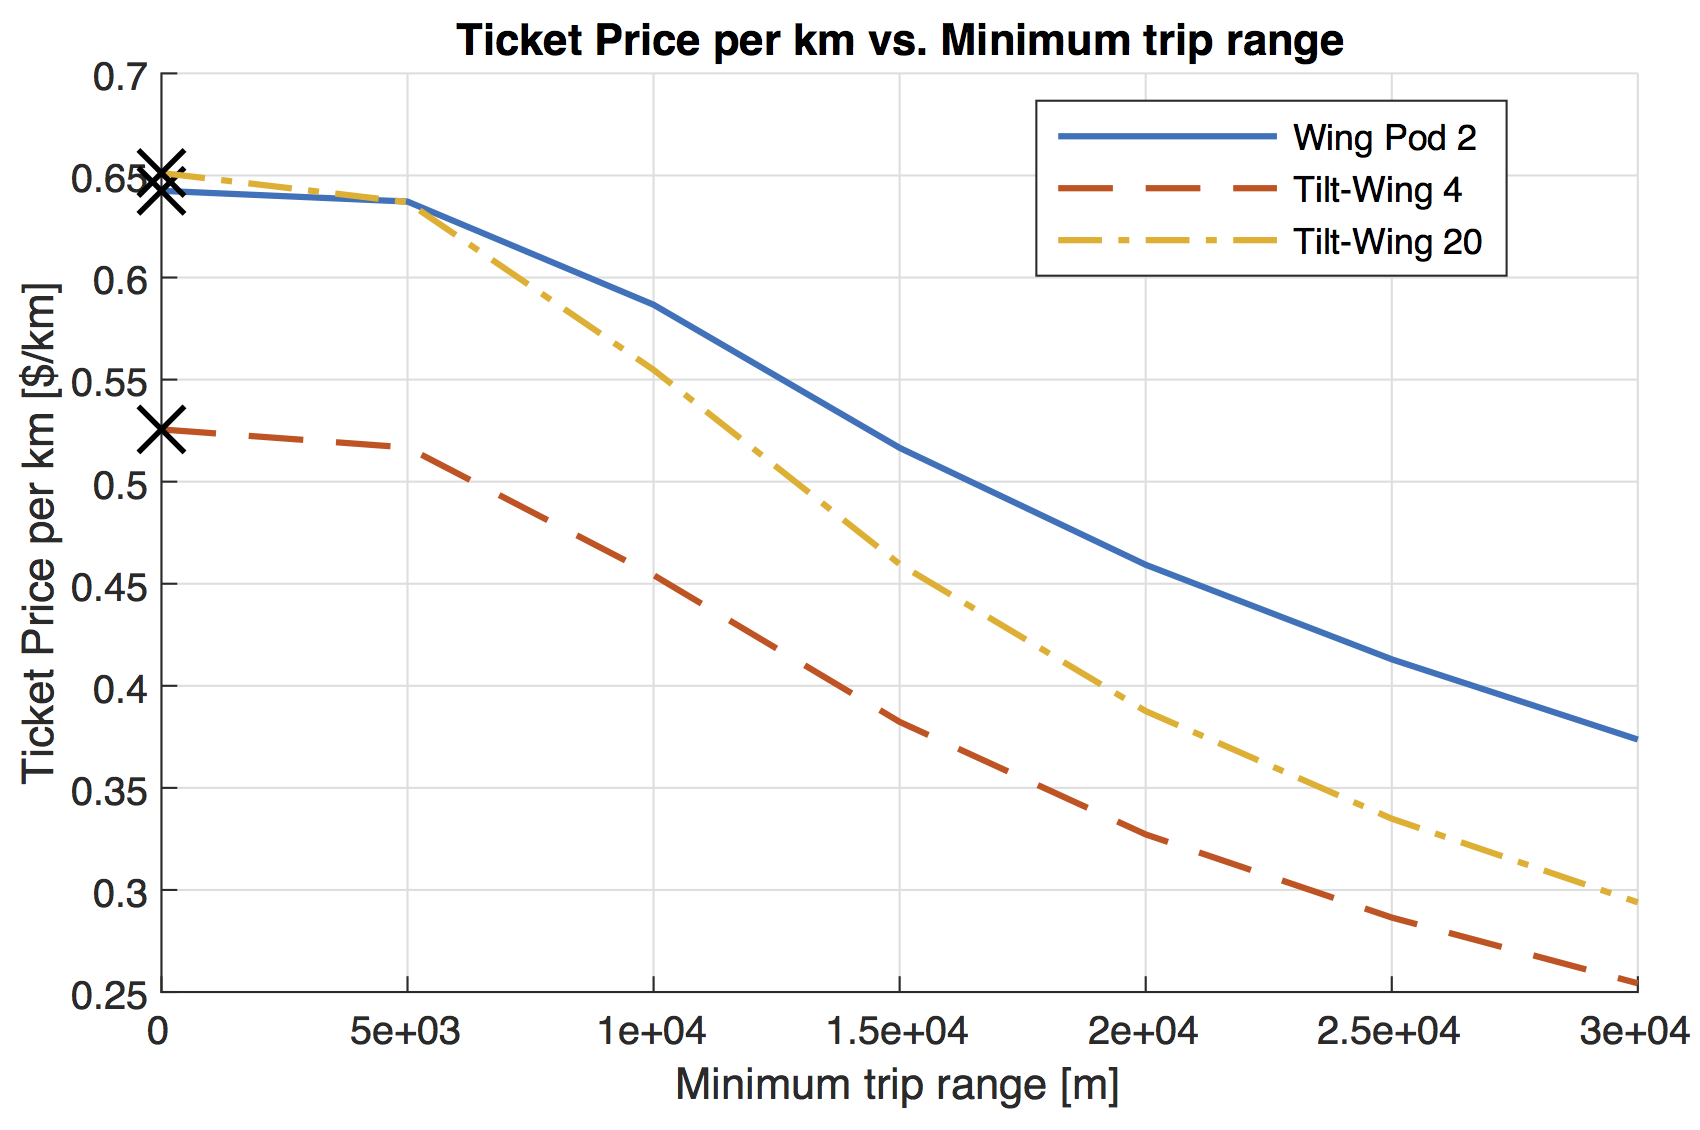
\includegraphics[width=\textwidth]{Figures/minRange_TPrice_perkmNOPAD.png}
    \captionsetup{justification=centering}
    \caption{Ticket price per km vs. Minimum range}
    \label{fig:sens02}
\end{subfigure}
\begin{subfigure}[t]{0.33\textwidth}
    \centering
    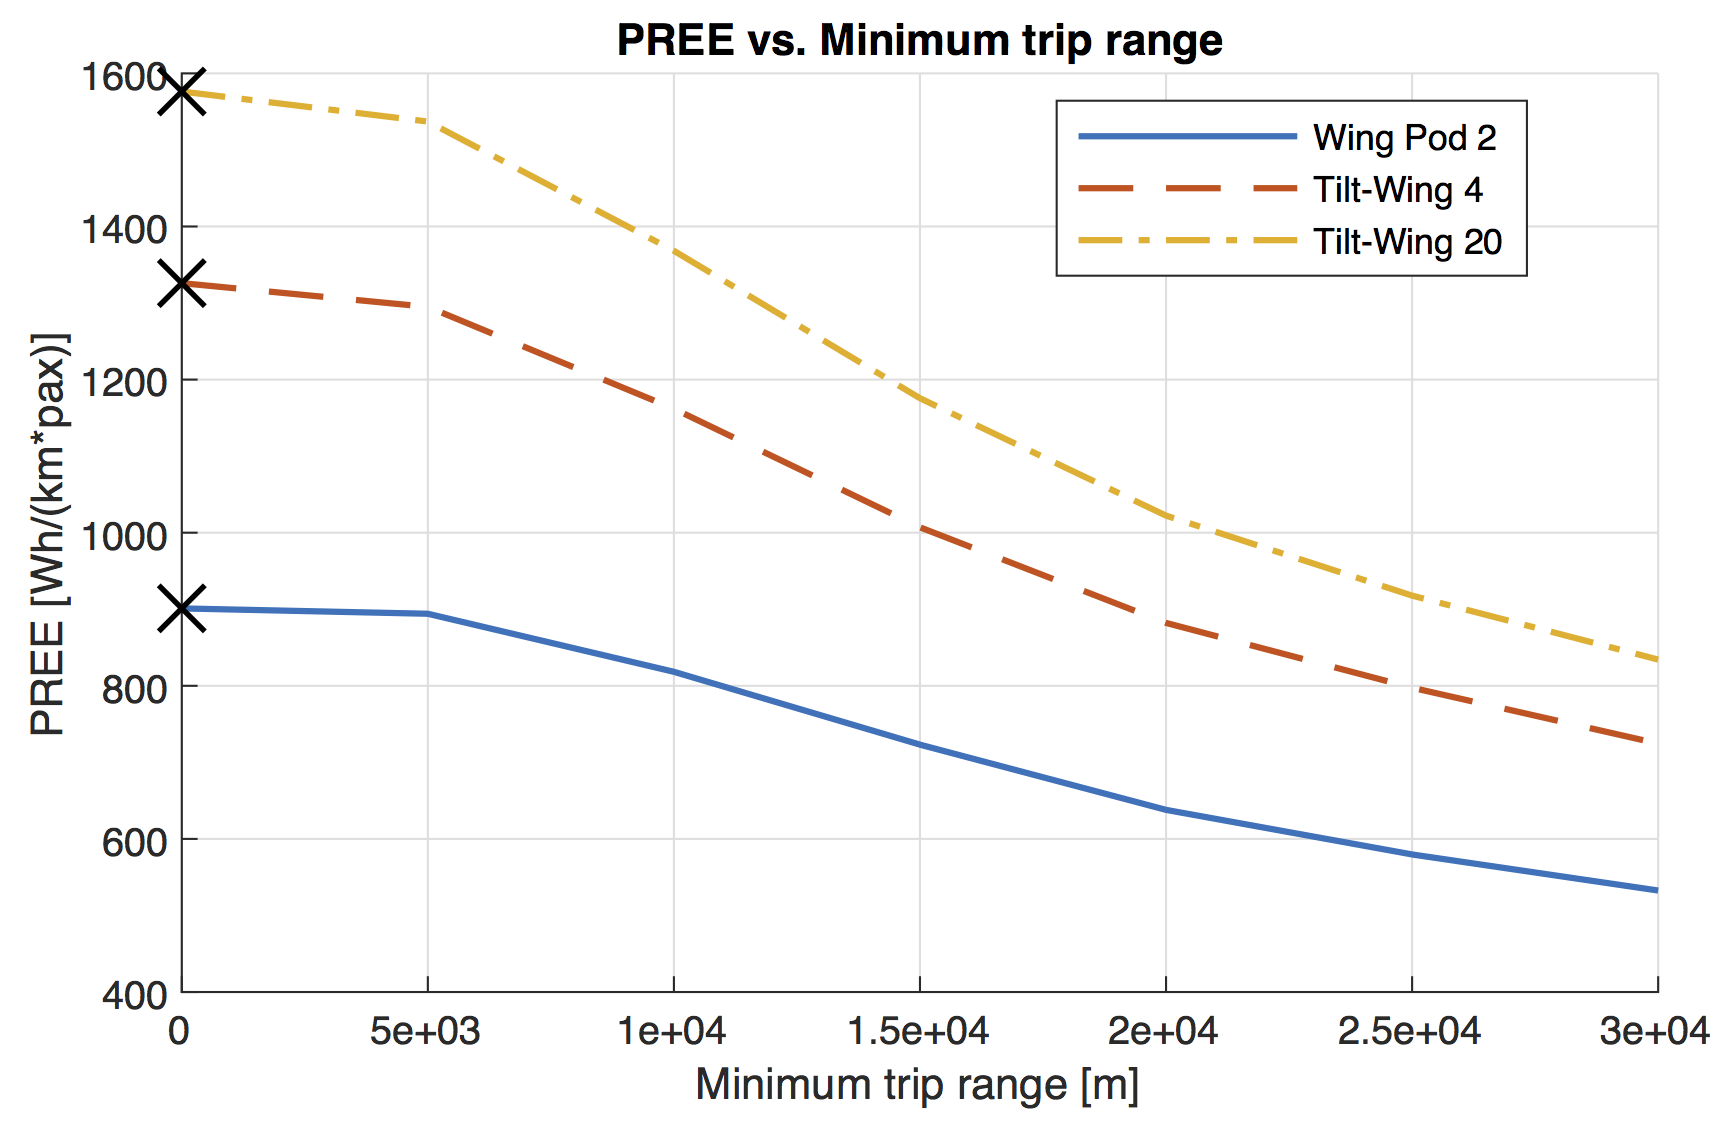
\includegraphics[width=\textwidth]{Figures/report_PREE.png}
    \captionsetup{justification=centering}
    \caption{Passenger range energy efficiency vs. Minimum range}
    \label{fig:sens03} 
\end{subfigure}
\captionsetup{justification=centering}
\caption{}
\label{fig:sens0123}
\end{figure}

\begin{figure}[h]
\begin{subfigure}[t]{0.33\textwidth}
    \centering
    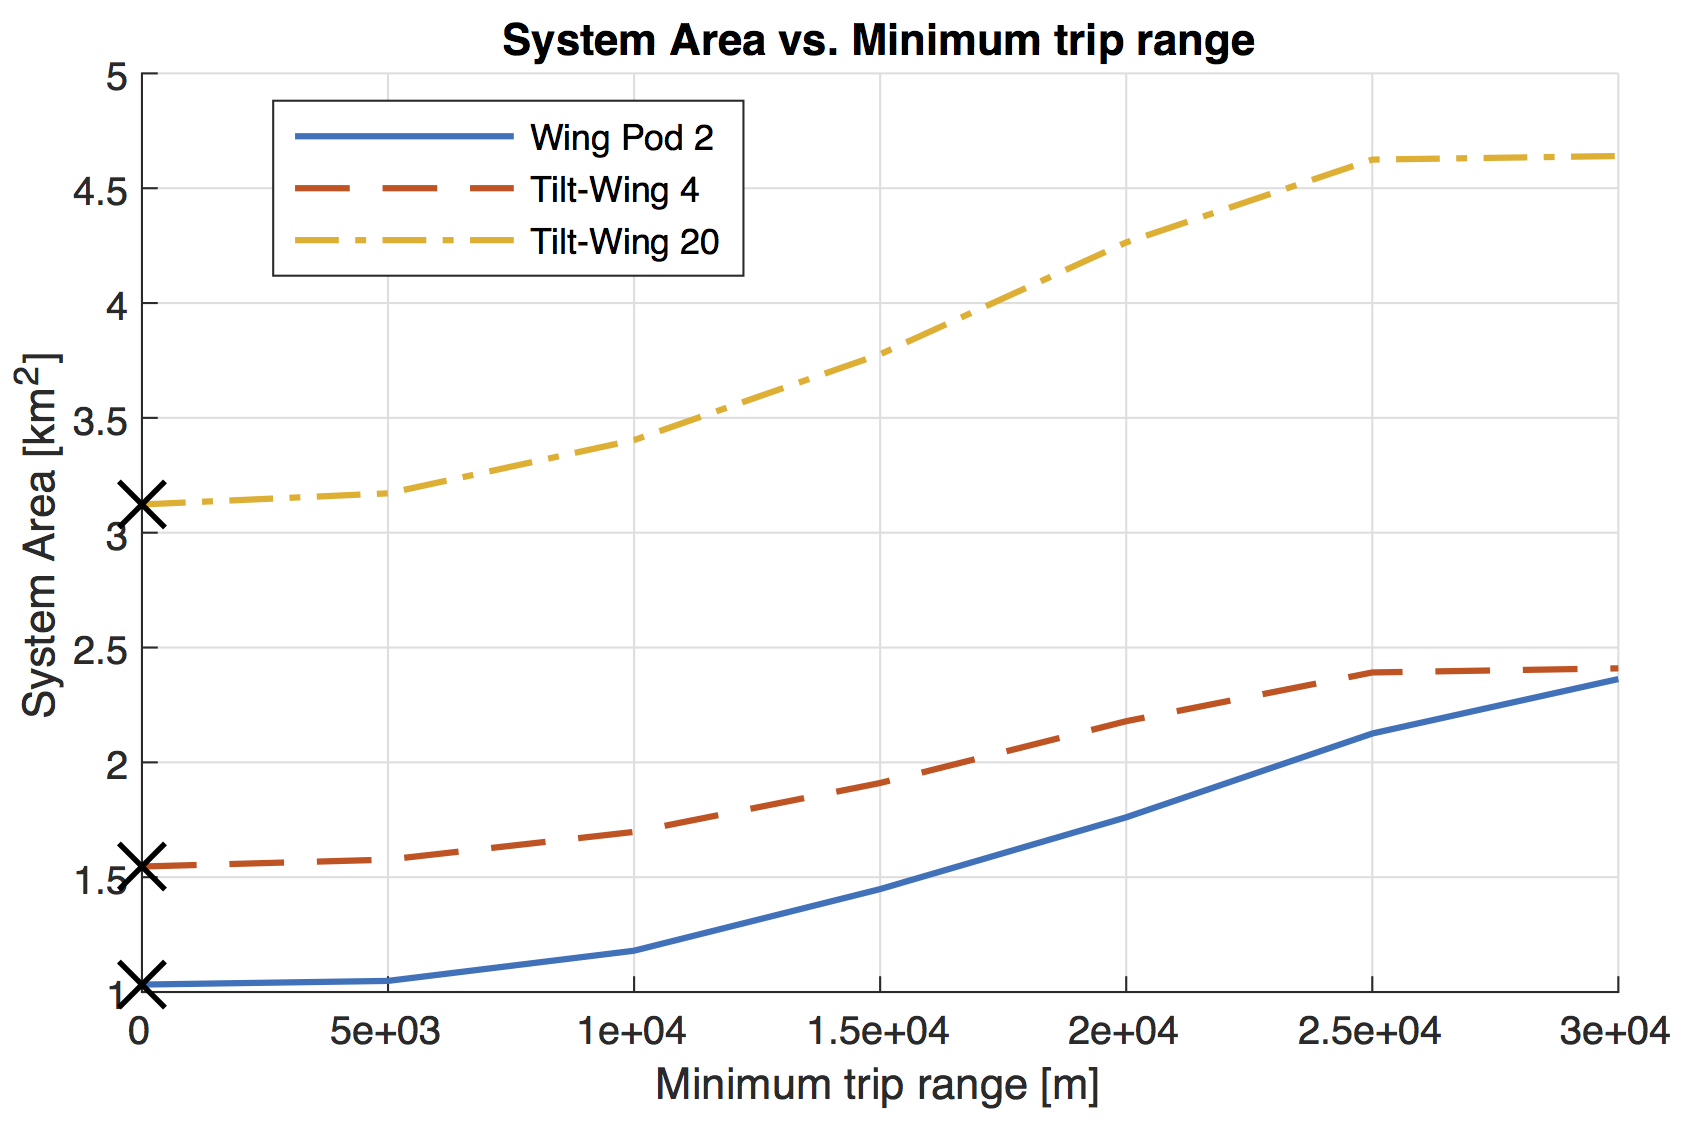
\includegraphics[width=\textwidth]{Figures/report_sys_area.png}
    \captionsetup{justification=centering}
    \caption{Total System Area vs. Minimum Range}
    \label{fig:sens1}
\end{subfigure}
\begin{subfigure}[t]{0.33\textwidth}
    \centering
    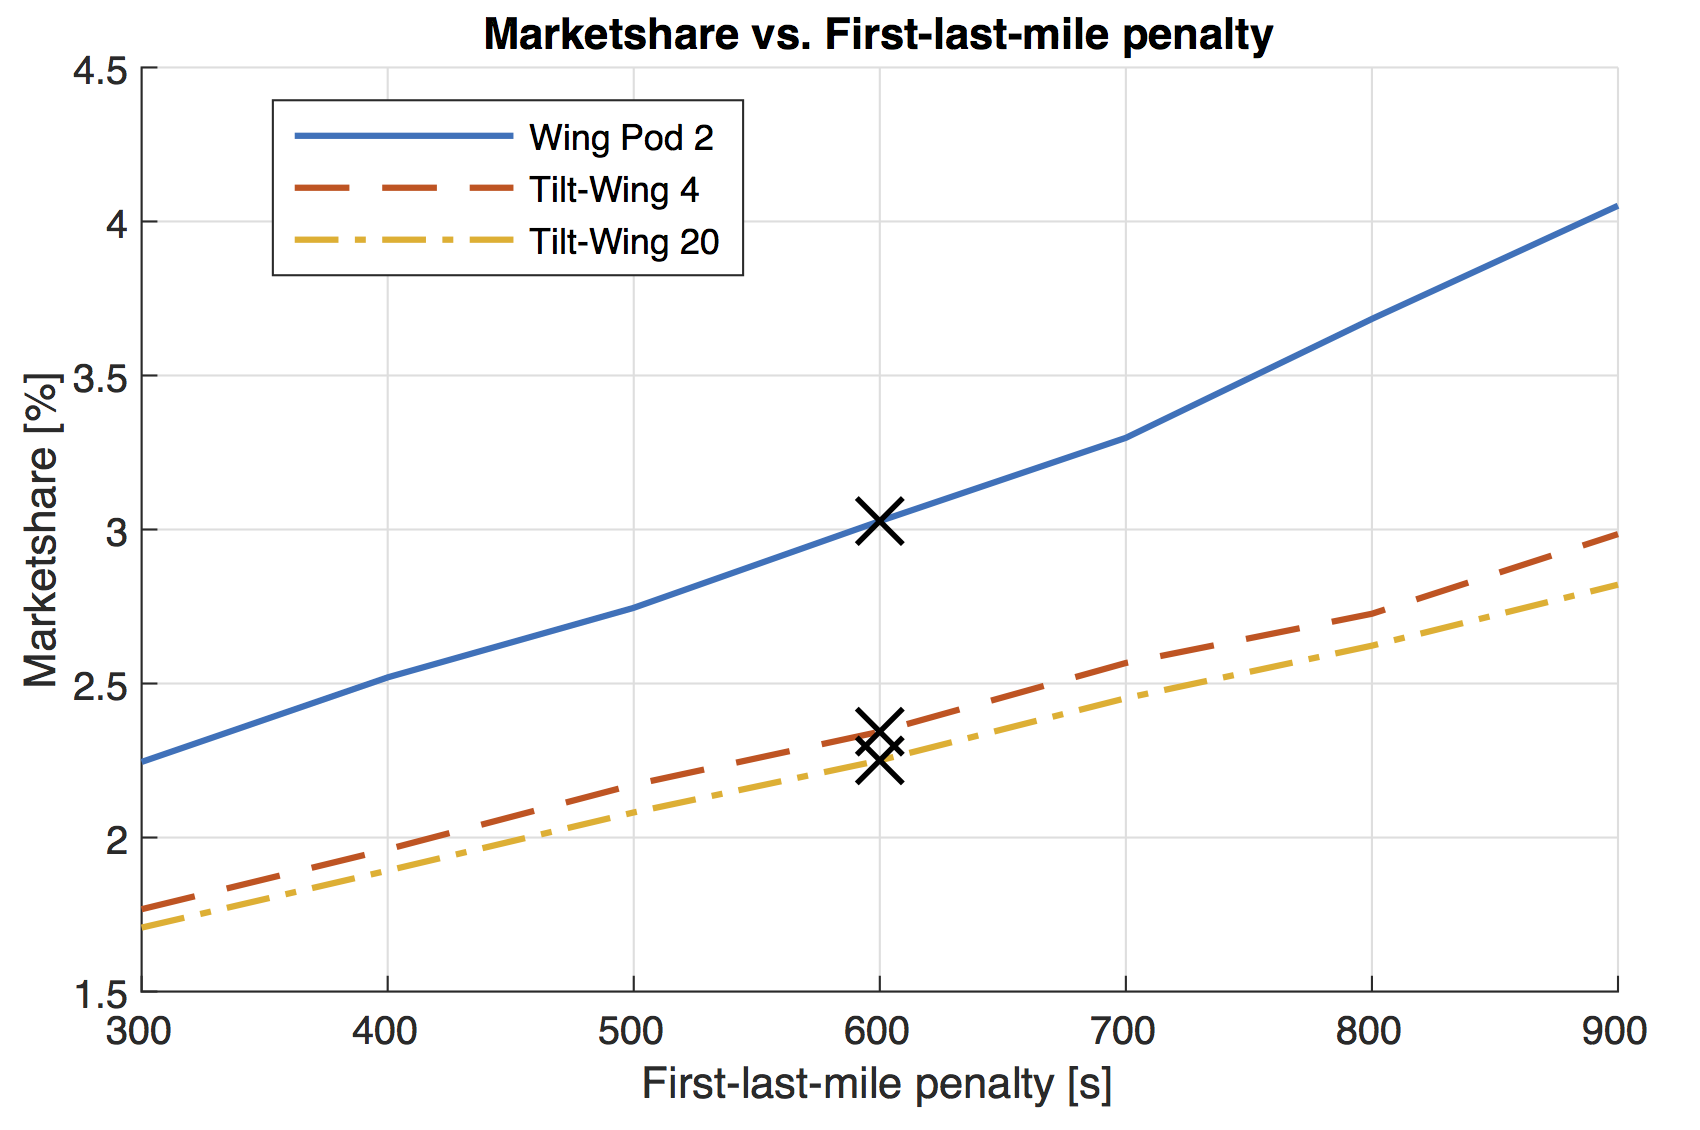
\includegraphics[width=\textwidth]{Figures/report_marketshare.png}
    \captionsetup{justification=centering}
    \caption{Market Share vs. Last-mile penalty}
    \label{fig:sens2}
\end{subfigure}
\begin{subfigure}[t]{0.33\textwidth}
    \centering
    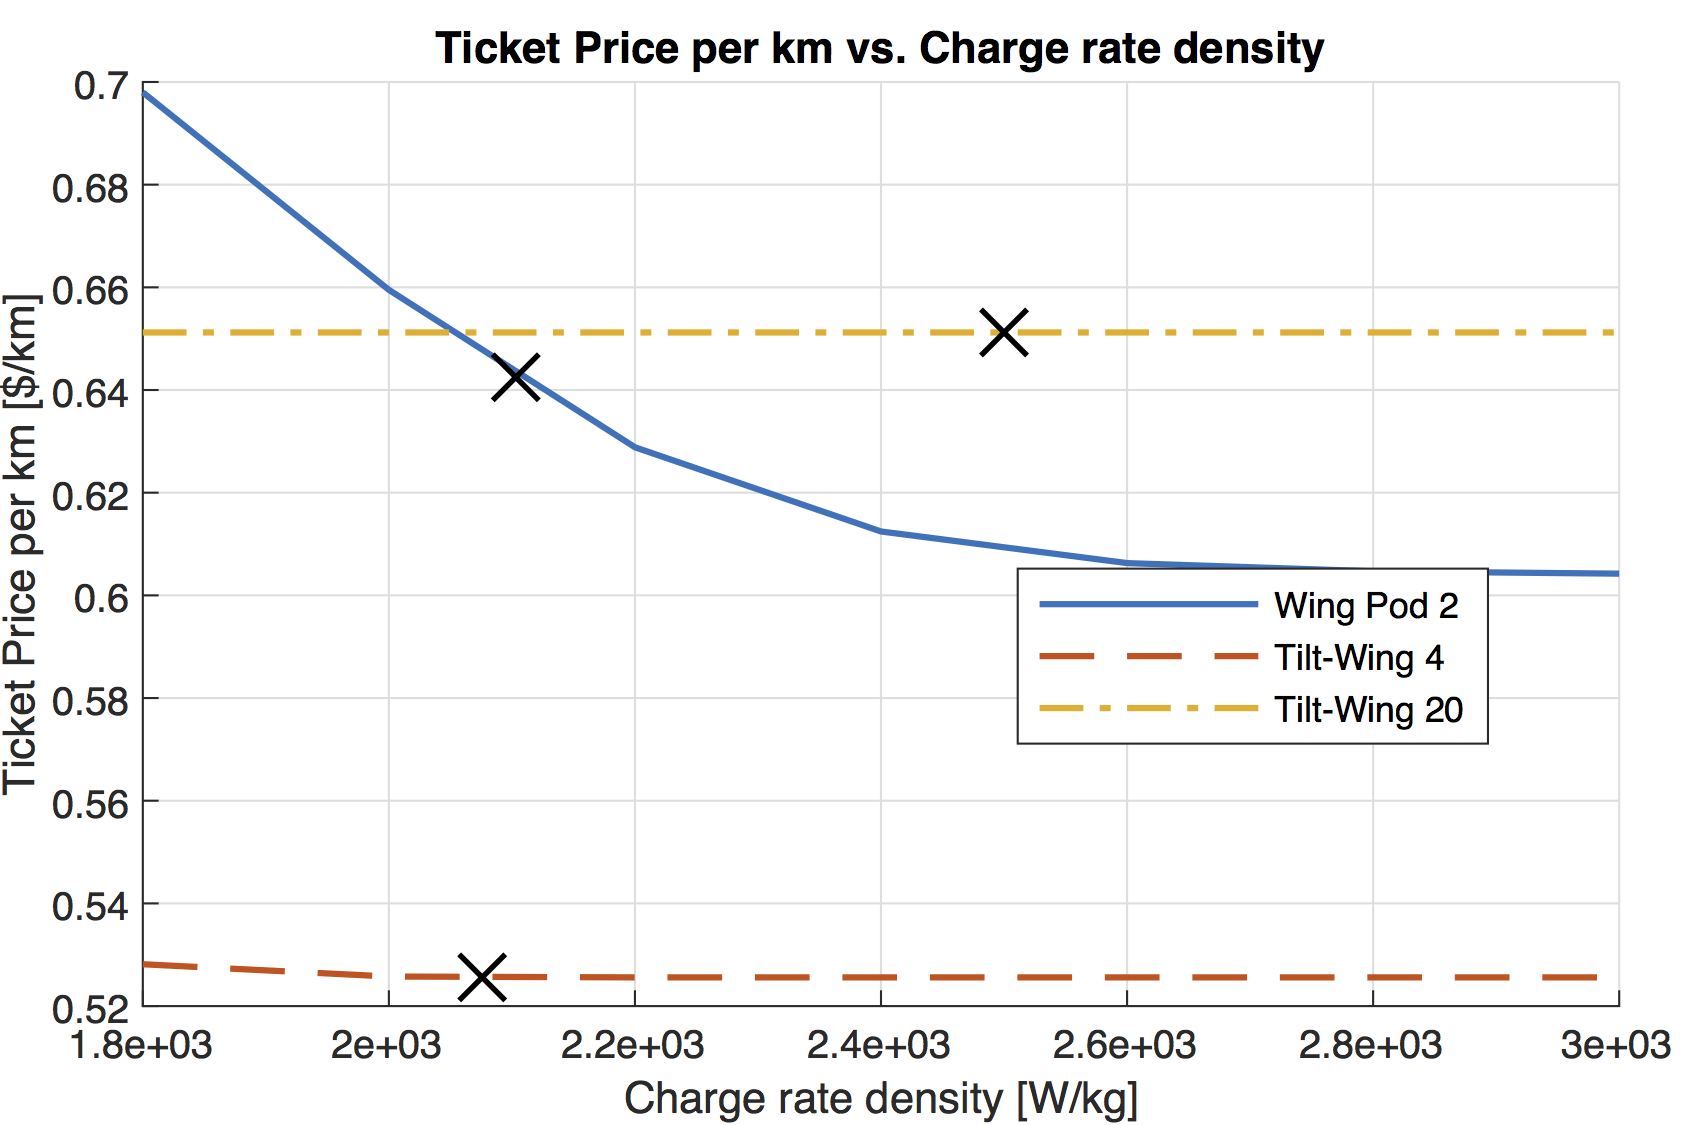
\includegraphics[width=\textwidth]{Figures/CRate_TPrice_perkmNOPAD.png}
    \captionsetup{justification=centering}
    \caption{Ticket price per km vs. Charge rate density}
    \label{fig:sens7}
\end{subfigure}
\captionsetup{justification=centering}
\caption{}
\label{fig:sens123}
\end{figure}


\subsection{Vehicle Weight and Energy Consumption}

\begin{figure}[h]
\begin{subfigure}[t]{0.33\textwidth}
    \centering
    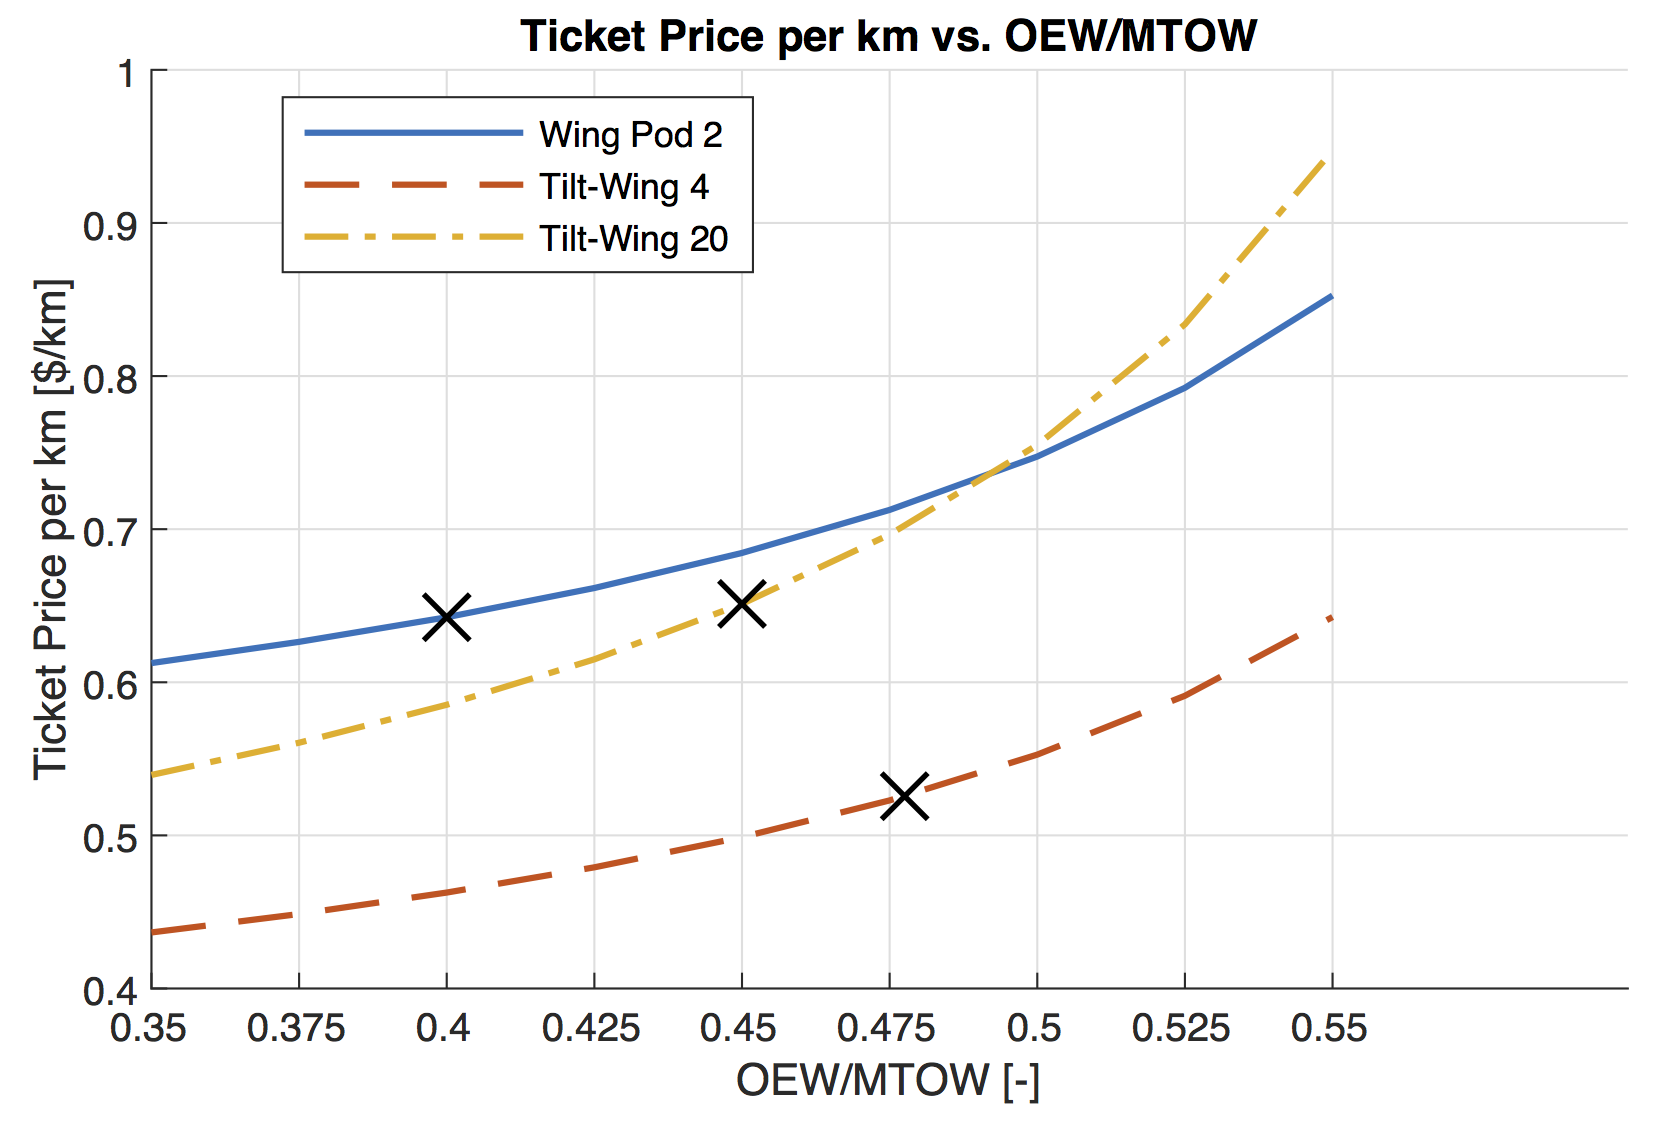
\includegraphics[width=\textwidth]{Figures/OEWMTOW_TPrice_perkmNOPAD.png}
    \captionsetup{justification=centering}
    \caption{Ticket price per km vs. OEW/MTOW ratio}
    \label{fig:sens4}
\end{subfigure}
\begin{subfigure}[t]{0.33\textwidth}
    \centering
    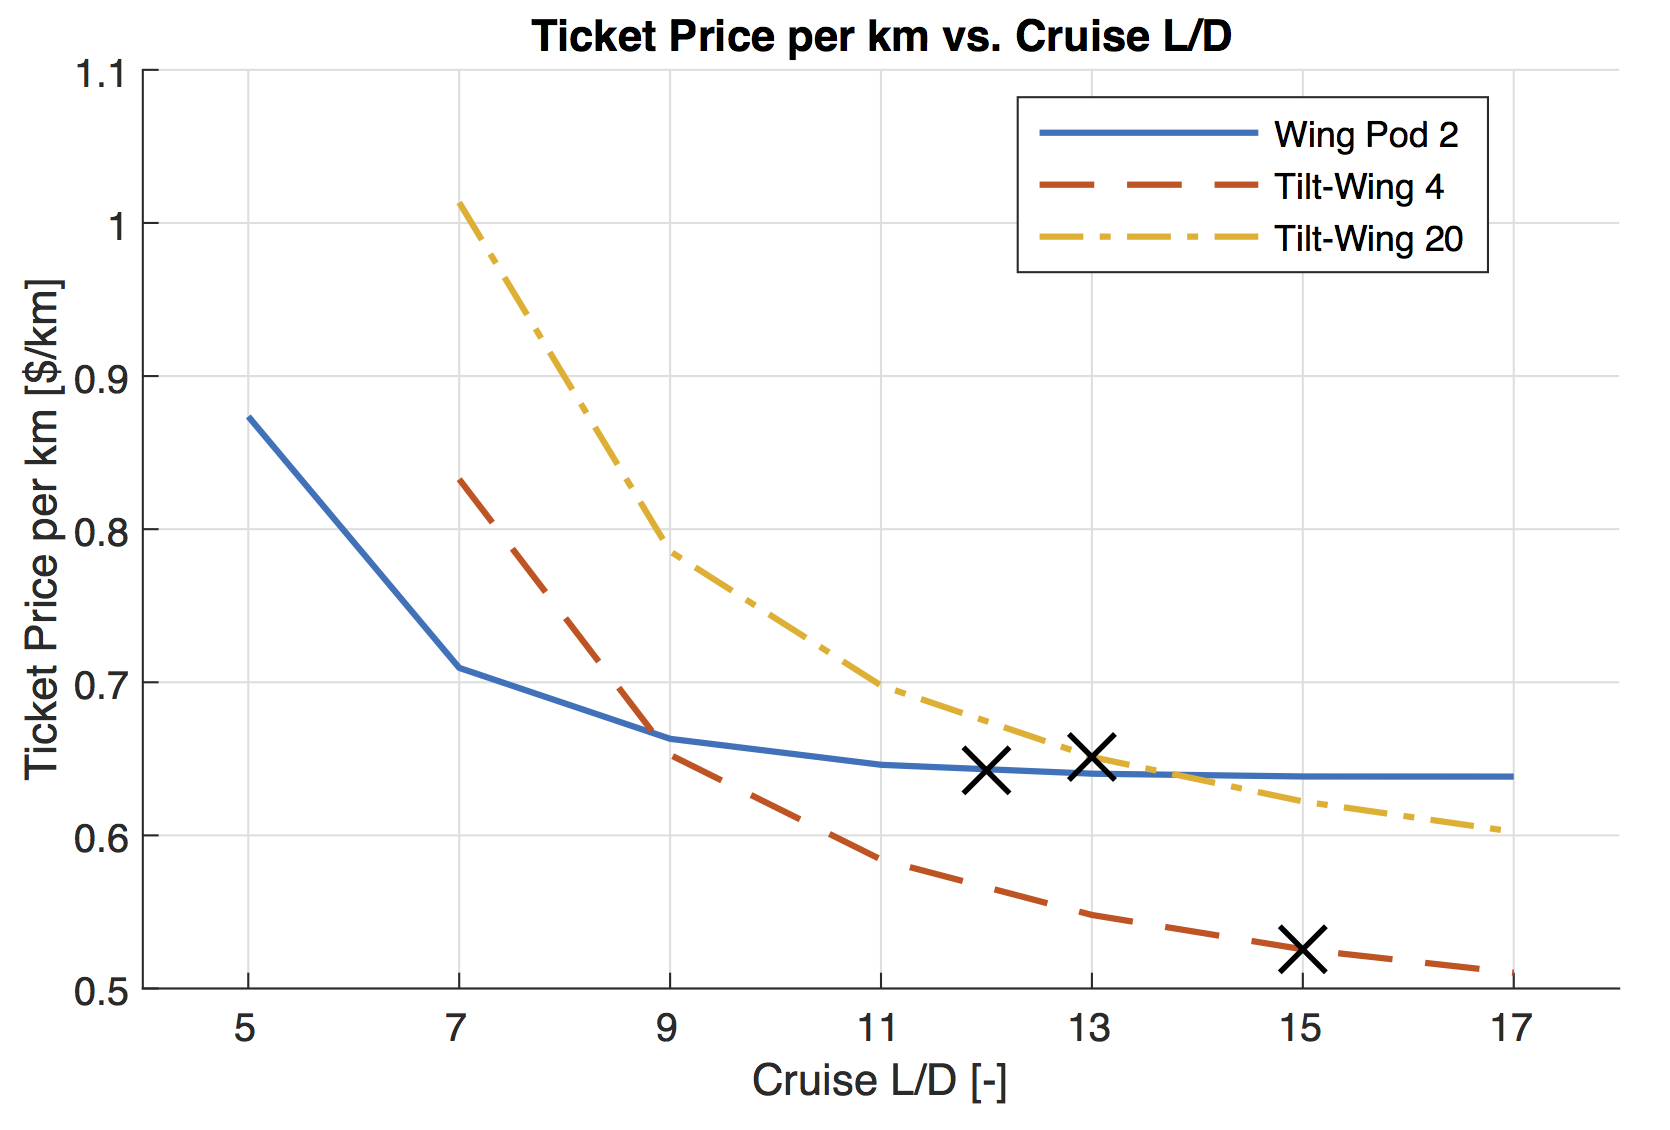
\includegraphics[width=\textwidth]{Figures/LoD_TPrice_perkmNOPAD.png}
    \captionsetup{justification=centering}
    \caption{Ticket price per km vs. L/D in cruise}
    \label{fig:sens5}
\end{subfigure}
\begin{subfigure}[t]{0.33\textwidth}
    \centering
    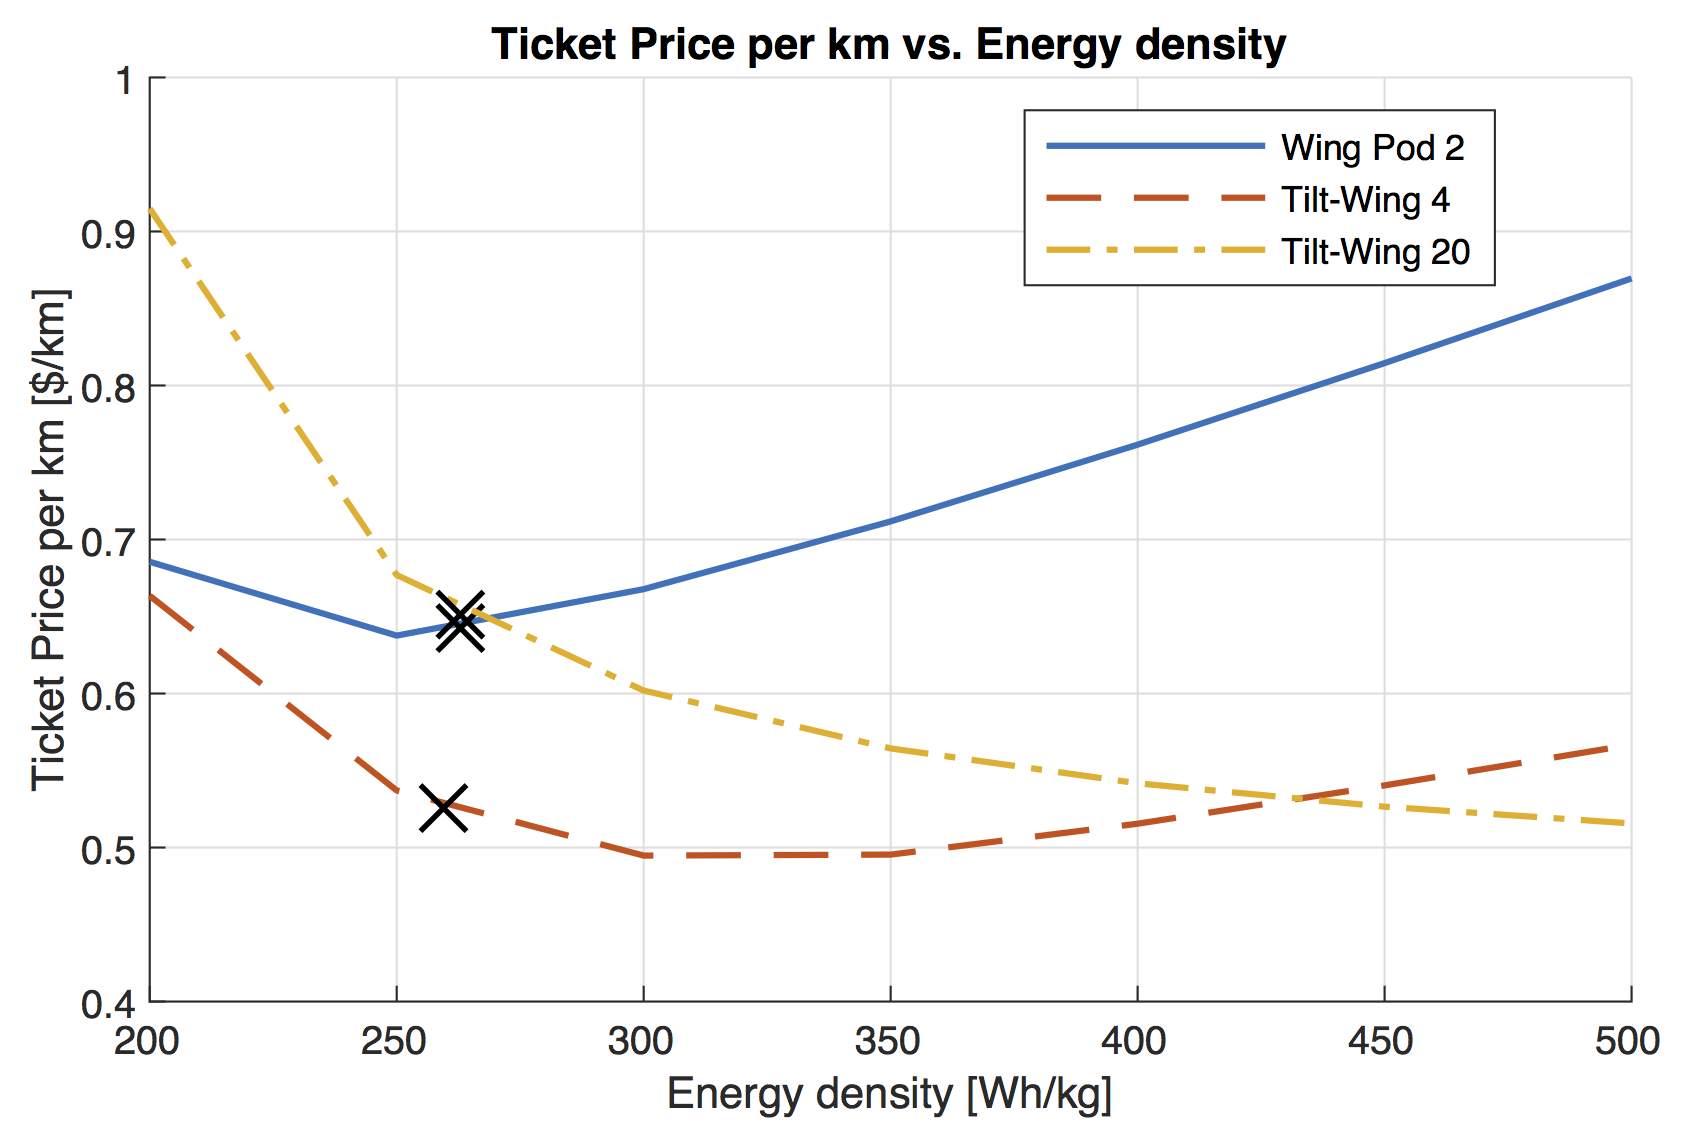
\includegraphics[width=\textwidth]{Figures/Edens_TPrice_perkmNOPAD.png}
    \captionsetup{justification=centering}
    \caption{Ticket price per km vs. Battery energy density}
    \label{fig:sens6}
\end{subfigure}
\captionsetup{justification=centering}
\caption{}
\label{fig:sens456}
\end{figure}


Some sensitivities are intuitively explained and verify the correct working of the tool. For example, an increase in the fraction of empty and maximum operational mass causes a higher ticket price. The heaviest vehicle is effected most by that effect as can be told by comparing the slopes in figure \ref{fig:sens4}. A more efficient cruise causes the energy consumption to be lower which also decreases OEW (OEW is considered an output of the tool here, since it is converged on every run). 

Counter intuitive is that ticket price can increase with increasing energy density. This does not seem to make sense at first. However, consider that charge rate density (expressed in W/kg) is kept constant when energy density is perturbed. Recall, that the batteries recharging time is modelled as inversely proportional to the charge rate and proportional to the energy needed for every given trip. Since the chosen vehicles are energy limited (not power limited) during take off, this means that battery mass decreases as energy density increases. However, the trip energy demand does not vary linearly with the battery mass. It varies approximately as $MTOW\sqrt{MTOW}$ during the hovering phases, as opposed to the charge rate, which \emph{is} inversely proportional to the battery mass \autoref{eq:power}\autoref{fig:sens7}. This way, charge time actually increases, because the increase in charge rate with battery mass is lower than the increase in energy demand with battery mass. Therefore, a longer turnaround time is needed for recharging which necessitates a bigger fleet and more vertiports for the same passenger throughput. This means that we will have to find battery technology that does not just increase energy density, since a smaller battery does not necessarily improves economic performance; a very interesting result. The reason that the 20 person vehicle in \autoref{fig:sens6} is not following this trend is because the turnaround time is limited by boarding procedures, not charging time. So a longer charging time does not deteriorate ticket price. The bottom line to this is that optimisation for the smallest necessary battery weight, as done in tool, may not yield the lowest ticket price even if it improves sustainability through less battery mass and lower energy usage per passenger kilometre.

Also; not shown here, the system area increases for a higher L/D. If pad infrastructure costs are higher than shown here, the sensitivity in L/D can reverse. So a higher L/D actually increases ticket prices, if optimisation for the lightest possible MTOW is performed, as usual. Compare with \autoref{fig:sens5}.

Even though counter-intuitive, the plots makes sense, taking into account the methods and calculations applied in the tool, which strengthens out faith in the tool.


\begin{wrapfigure}[13]{r}{0.35\textwidth}
    \centering
    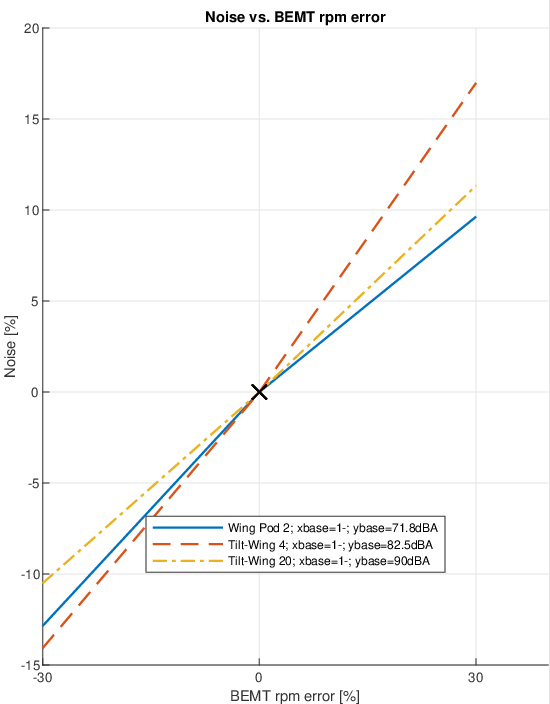
\includegraphics[width=0.35\textwidth]{Figures/NoiseBEMT.PNG}
    \captionsetup{justification=centering}
    \caption{BEMT RPM error propagation onto Noise}
    \label{fig:BEMTerror}
\end{wrapfigure}

\section{Impact of Tool Inaccuracies} \label{sec:errorSensitivity}

%\section{Error Sensitivity for Analysing Assumptions} 


Using the same sensitivity plot framework (\autoref{sec:sensitivityplot}) as in the above section, an easy-to-implement approach to tracking errors due to simplified calculations was developed. The earliest affected intermediate tool output is multiplied by a factor close to one and the sensitivity of the output criteria plotted against that factor. The severity of having an inaccurate method for that particular aspect of the tool can be evaluated by combining the change in the output with knowledge of the weight given to it in the trade off.

As an example, the propagation of an error in the rotor RPM as computed from the BEMT and its effect on noise is analysed; see \autoref{fig:BEMTerror}.



Now, of course the Noise increases with additional (artificial) RPM, but it is interesting to not that the sensitivities differ per concept. If the 4 pax concept is chosen, more attention needs to be paid at reducing the error in rpm, because the noise (which is an important criterion) would otherwise by over or underestimated, depending on the sign of the error.




\section{Design Validation using Statistics} \label{sec:statsVal}

Even at this stage of the most top level concept design, it is useful to compare the outputs with known similar concepts as an intermediate validation level. This helps evaluating if the combination of parameters are realistic and feasible. In \autoref{fig:MTOW-Pax2} and \autoref{fig:Cruise-MTOW2}, the same statistical plots from \autoref{subsec:desvector} are given with the concepts included as light-blue diamonds. For both, they fall within realistic margins as shown in \autoref{fig:MTOW-Pax2} and \autoref{fig:Cruise-MTOW2} respectively. The range of many of the reference vehicles was reduced according to the market needs. This results in lower battery mass, which accounts for some difference from statistics, but still results in feasible design options. 

The larger 20 person vehicles do not fall within any available statistics, as there are simply no existing vehicles in this category, so no validation of this kind can be performed.

\begin{figure}[H]
\begin{subfigure}[t]{0.5\textwidth}
    \centering
    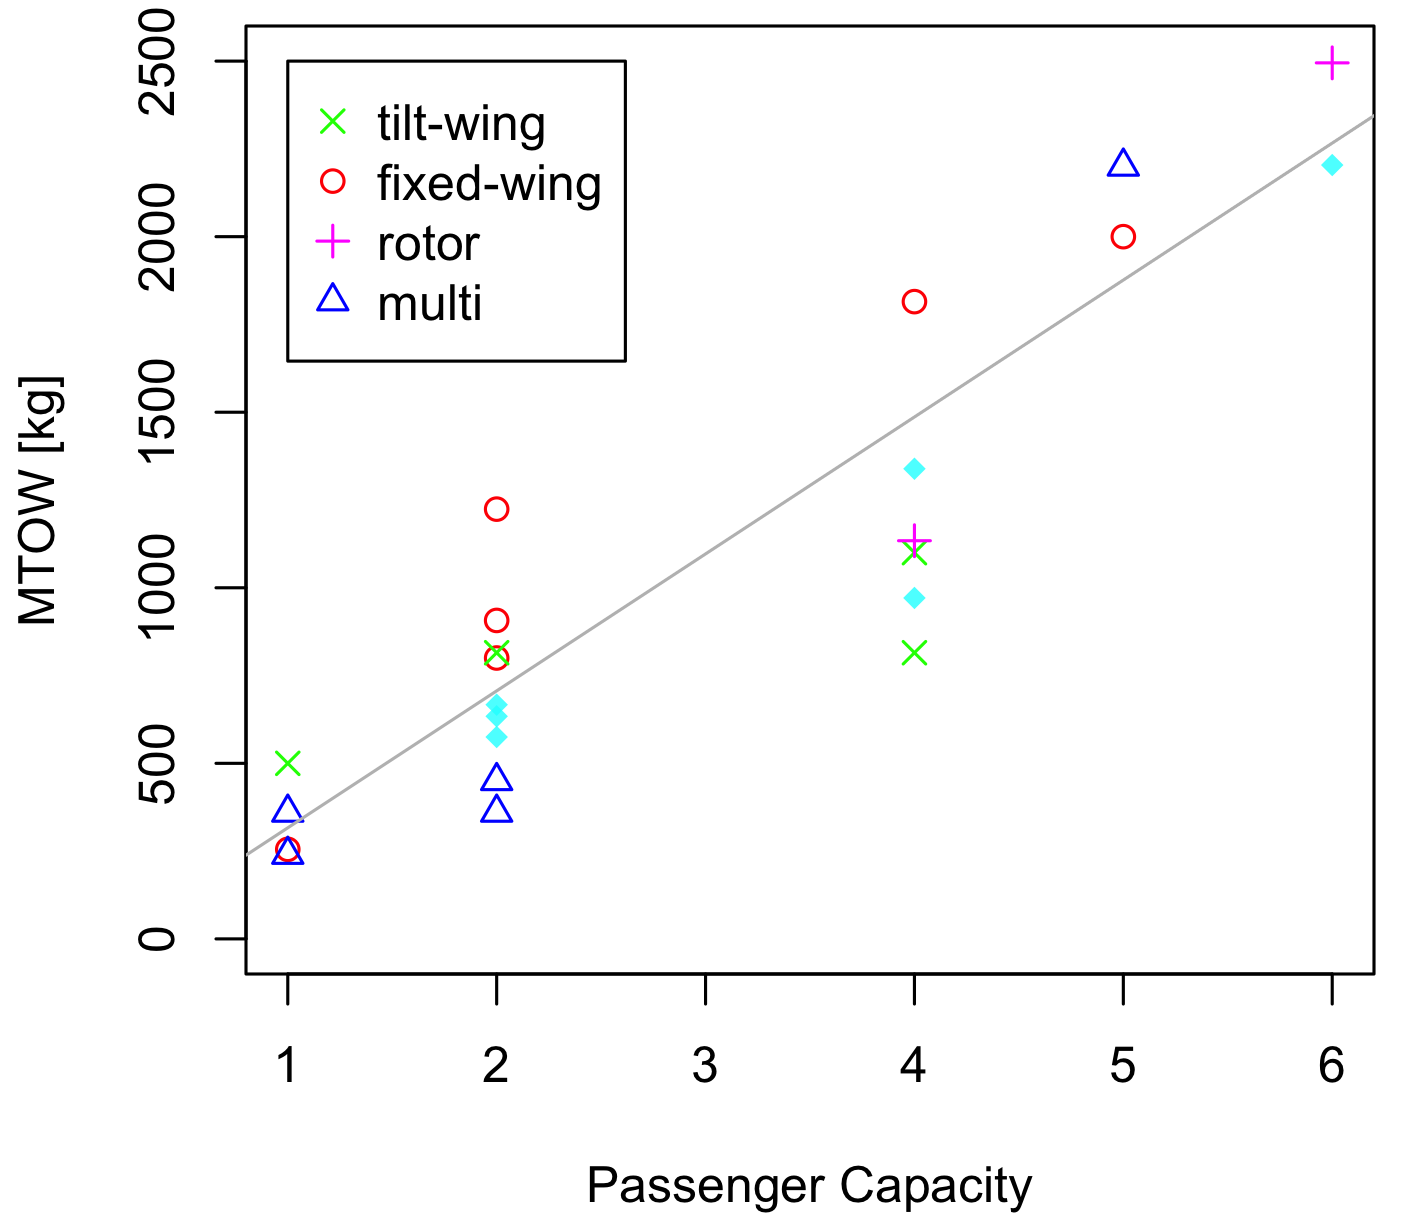
\includegraphics[width=\textwidth]{Figures/MTOW-Pax2.png}
    \captionsetup{justification=centering}
    \caption{When comparing MTOW to number of passengers, the designed concepts (blue diamonds) fit with existing statistics.}
    \label{fig:MTOW-Pax2}
\end{subfigure}
\begin{subfigure}[t]{0.5\textwidth}
    \centering
    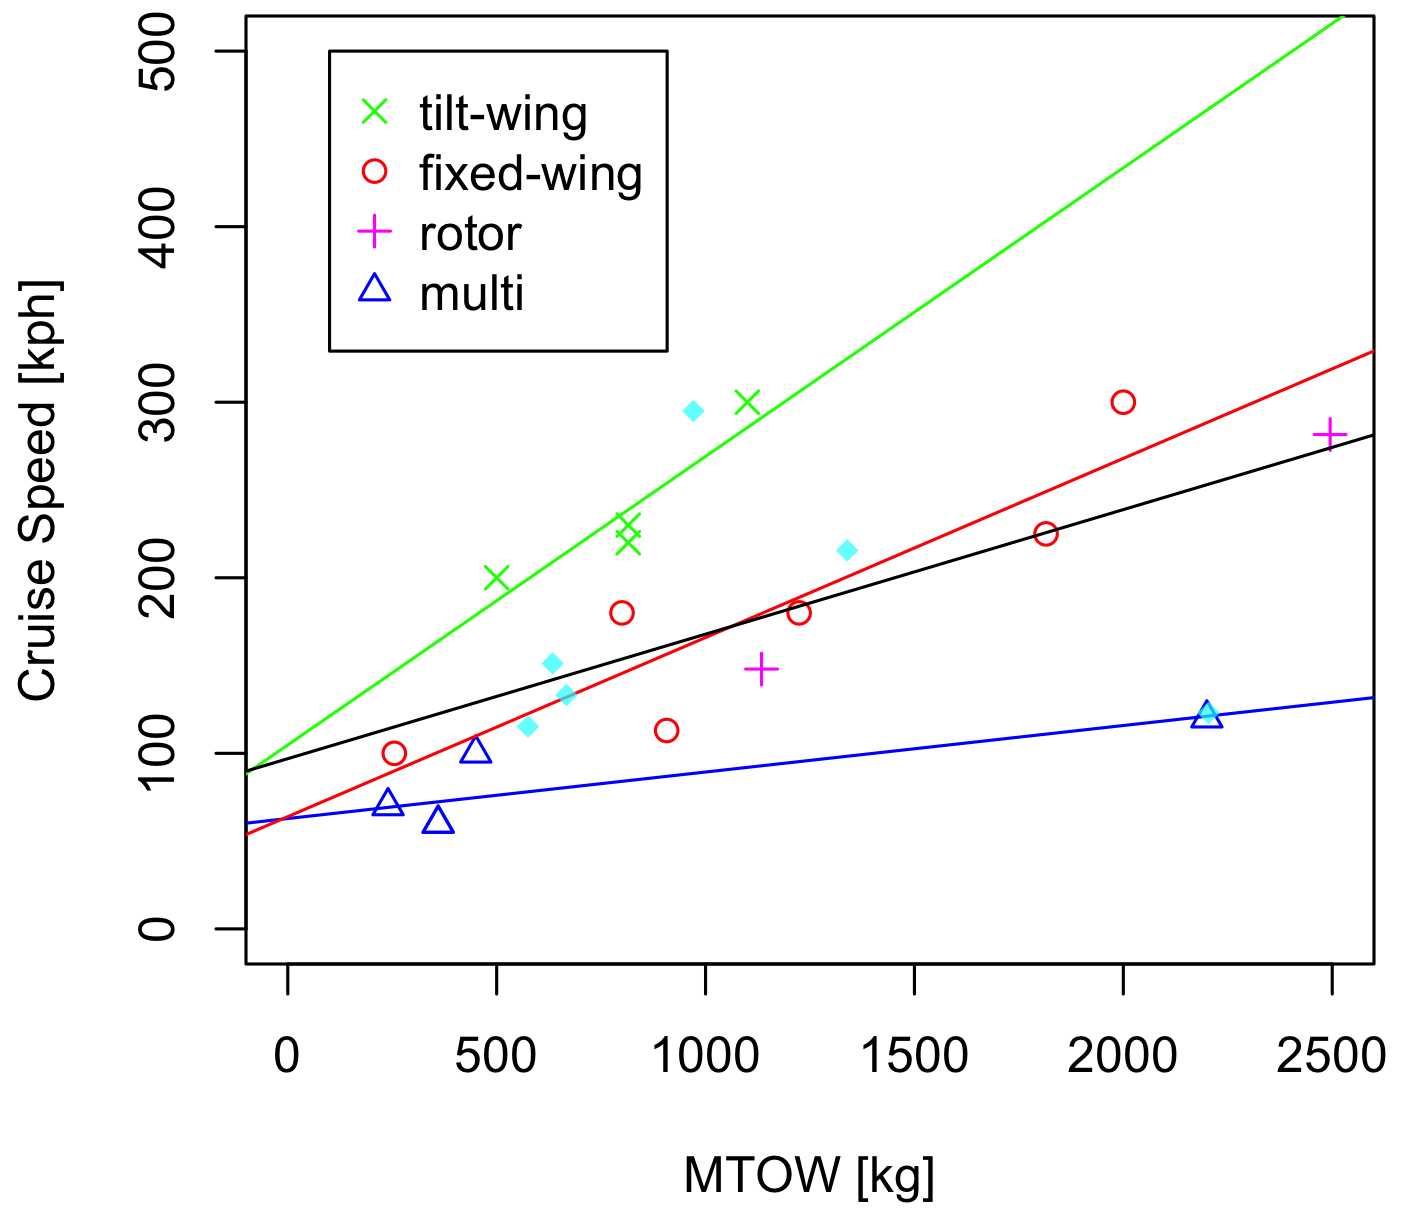
\includegraphics[width=\textwidth]{Figures/Cruise-MTOW2.png}
    \captionsetup{justification=centering}
    \caption{When comparing MTOW to cruise speed, the designed concepts (blue diamonds) fit with existing statistics.}
    \label{fig:Cruise-MTOW2}
\end{subfigure}
\captionsetup{justification=centering}
\caption{}
\label{fig:concept_compare}
\end{figure}
